% !TEX root = main.tex
\chapter{Results}\label{cha:result}
This section describes the results considering performance, robustness and stability with respect to the different control approaches. All approaches will first be benchmarked with the present control approach and presented individually in the following subsections. A comparison between all approaches is presented in the end of this chapter.

\section{Benchmark tests}
Each of the control approaches have been evaluated with respect to robustness to model errors, disturbance rejection, closed loop bandwidth and response to step, ramp and sinusoidal input, all summarized below. The prospective challenges, described in \ref{sec:prospectiveChallanges} shall be kept in mind while reading the results. Since the required ramp rates are relatively low, the disturbance rejection and the robustness to model errors are more of interest when evaluating each method.

\begin{itemize}
\item {\bf Step, ramp and periodical tracking} - A step, ramp and periodic input is applied on the input to benchmark the tracking capability of the controller.
\item {\bf Disturbance rejection} - Modified step responses with impulses added to the input and measurement signal to benchmark how sensitive the system is to system disturbances.
\item {\bf Robustness to model errors} - During operation with a periodic input signal, the dynamical model is changed and the output is studied to characterize the robustness to model errors. This test is of importance since this is exactly what happens when the linear stage moves the rotational stage further out.
\end{itemize}

\section{Linear dynamics characterization}
The linear dynamics of the rotational stage changes due to the a number of physical properties of the system, such as the current yaw-position, the linear axis position and speed and if the system is in contact with the end-switches. This phenomenas were characterized in a number of tests and summarized below. Figure~\ref{fig:different_angles} shows a comparison of the identified model when the linear axis is in its outer position and the rotational head has rotated 0 mrad (0V), 10 mrad (3.25V) and 20 mrad (6.5V). It shows that the system changes its first resonance peak as much as 5.3 Hz.

Figure~\ref{fig:different_lin_pos} shows a comparison of the identified model when the rotational head is in 10 mrad (3.25V) and the linear axis position is in 1, 20, 40 and 57mm. The identified system are almost the same for the first 3 positions, but it changes drastically when the linear axis touches the outer switches in 57mm.

\begin{figure}[h!]
  \centering %crop: left bottom right top
  \subfloat[][\label{fig:different_angles}Zoom in]{
  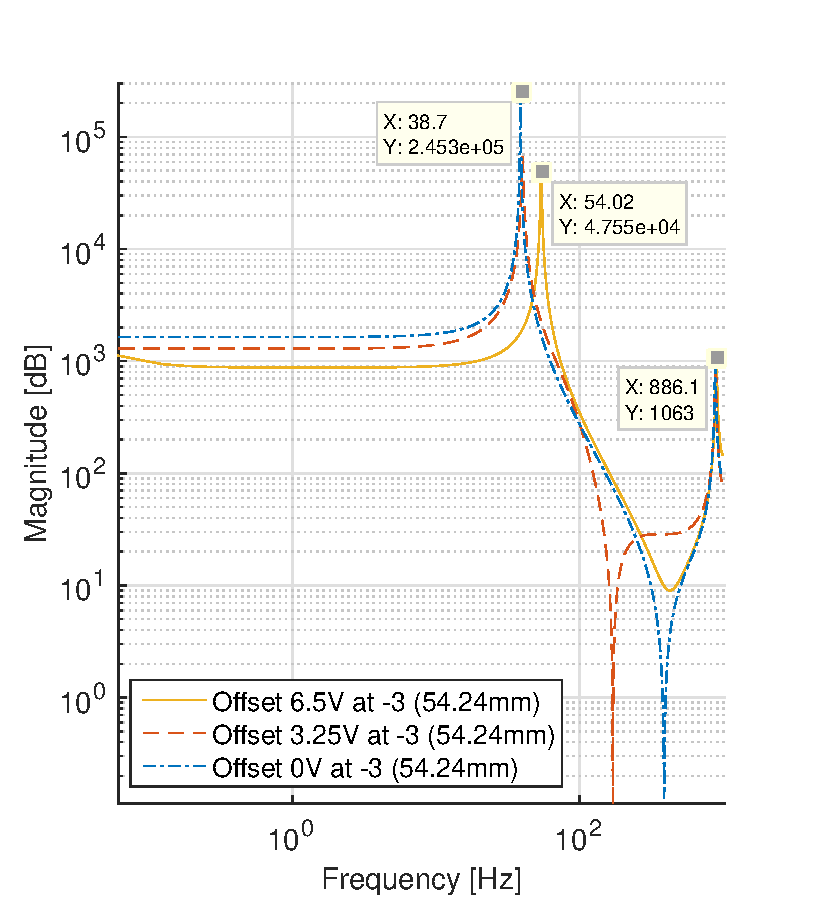
\includegraphics[width=0.46\textwidth, trim=0cm 0cm 0.8cm 0cm, clip=true]{fig/matlab/modelcomparison_diffvolt2.eps}}
  \qquad
  \subfloat[][\label{fig:different_lin_pos}Open loop response]{
  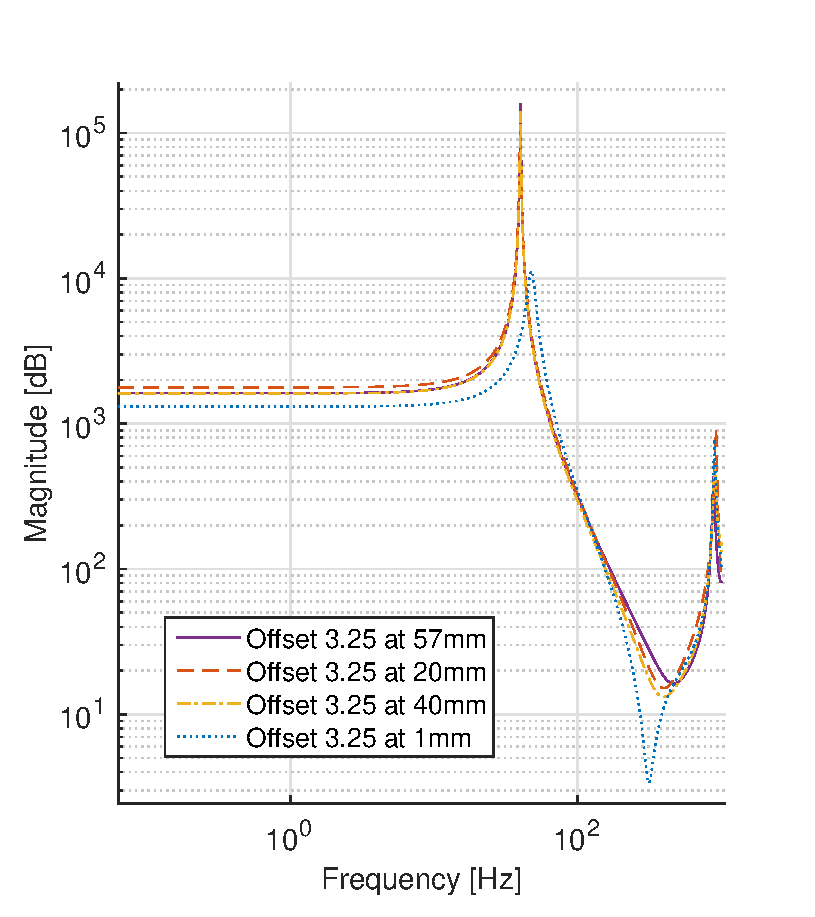
\includegraphics[width=0.46\textwidth, trim=0cm 0cm 0.8cm 0cm, clip=true]{fig/matlab/modelcomparison2.eps}}
  \caption{\label{fig:different_lin_angle} The resulting responses is shown in (a) with the model change in (b).}
\end{figure}

Since the rotational stage controller needs to maintain the required tracking error even when the linear axis is moving, the disturbance during linear operation must be considered. Figure~\ref{fig:dist_diff_speed} shows the open loop response when the linear axis is moving. This figure shows how the operating speed of the stepping motor influences the spectrum of the angle with its different harmonics.

\begin{figure}[h!]
  \centering %crop: left bottom right top
  \subfloat[][\label{fig:dist_diff_speed_overview}Open loop response]{
  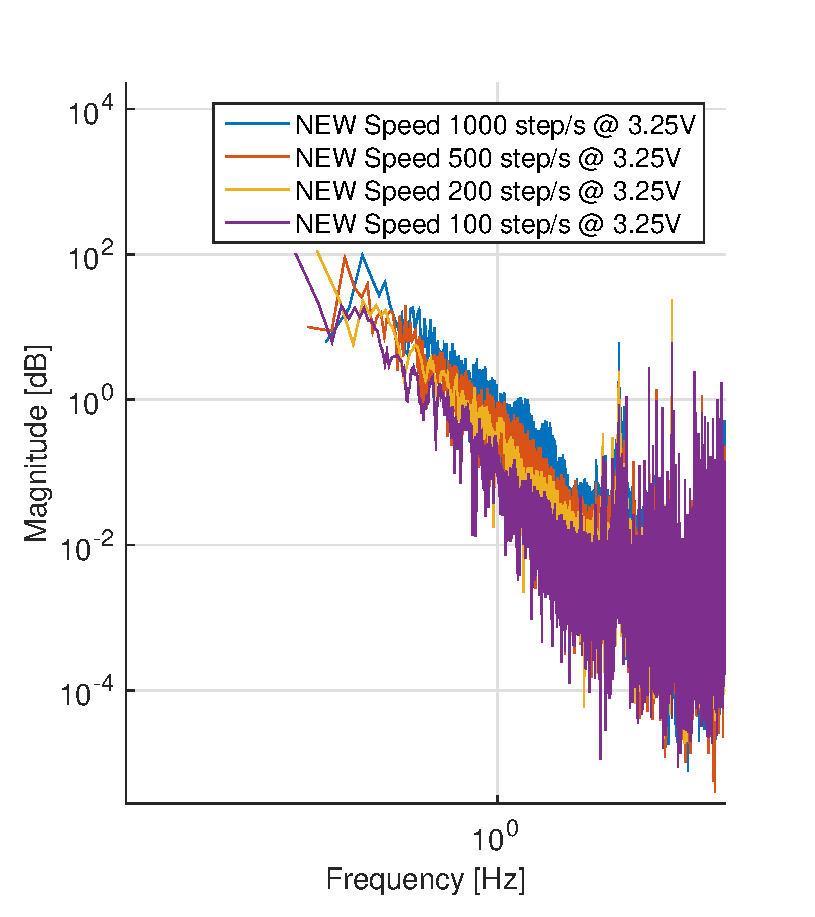
\includegraphics[width=0.46\textwidth, trim=0cm 0cm 0.8cm 0cm, clip=true]{fig/matlab/differentspeeds2.eps}}
  \qquad
  \subfloat[][\label{fig:dist_diff_speed_zoomin}Zoom in]{
  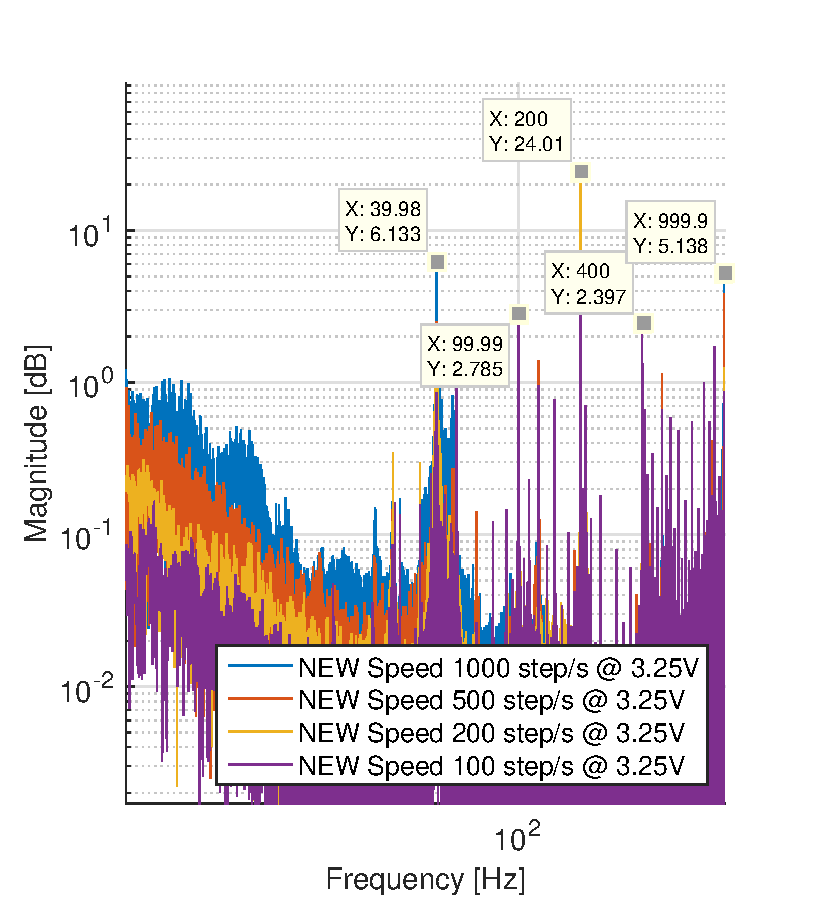
\includegraphics[width=0.46\textwidth, trim=0cm 0cm 0.8cm 0cm, clip=true]{fig/matlab/differentspeeds_Zoomin2.eps}}
  \caption{\label{fig:dist_diff_speed} The resulting responses is shown in (a) with the model change in (b).}
\end{figure}

\section{Simulation Results}
For the comparison with the present control approach, all evaluated controllers were discretized with a sampling frequency of 2kHz. A normalized version of the high order system in \eqref{eq:tf} was used to model the rotational stage linear dynamics. The nonlinear dynamics, creep and hysteresis, were neglected in the simulations, assuming perfect inverse hysteresis cancellation and a sufficient closed loop to compensate for the creep effect. All simulations were performed in Matlab and Simulink.

\subsection{Model Reference Adaptive Control}
Even though the rotational stage has been modeled by \eqref{eq:tf}, a second order model approximating the higher order system was used in the adaptive control laws to keep the computational burden low. The discretized reference model can be seen in \eqref{eq:sys_gm} and all parameters and tuning variables is summarized in Table~\ref{tab:adaptive_param}. The controller is tuned to be robust to input disturbances and model changes. The set of parameter presented in Table~\ref{tab:adaptive_param} is not an optimal set but a decent set of parameters that maintains stability for step sizes below 20mrad.

\begin{equation}
  \label{eq:sys_gm}
  G_m(z) = \frac{7.9z + 6.7}{1313z^{2} - 2095z + 796.4}
\end{equation}

\begin{table}[h!]
  \centering
  \begin{tabular}{| l | l |}
    \hline
    Parameter & Value \\ \hline
    $T_s$ & $5 \times 10^{-4}$ \\
    $\alpha_0$ & $5.7 \times 10^{4}$ \\
    $\alpha_1$ & $7.2$ \\
    $\beta_0$ & $7.5 \times 10^{7}$ \\
    $a_0$ & $5.7 \times 10^{4}$ \\
    $a_1$ & $1 \times 10^{3}$ \\
    $b_0$ & $7.5 \times 10^{7}$ \\
    $\eta_0$ & $3 \times 10^{-2}$ \\
    $\eta_1$ & $1 \times 10^{-1}$ \\
    $\eta_2$ & $1 \times 10^{-10}$ \\
    $\eta_3$ & $1 \times 10^{-17}$ \\
    $\epsilon$ & $1 \times 10^{-8}$ \\
    $Q$ & $diag(1 \times 10^{10}, 1 \times 10^{-3})$\\
    \hline
  \end{tabular}
  \caption{\label{tab:adaptive_param} Parameters of the system model and the tuned adaptive controller.}
\end{table}

Figure~\ref{fig:step_adaptive} shows the step response to different step sizes. Here it is clear that the system becomes unstable if the step size $\geq$ \unit{26}{\milli\radian}. The controller has been tuned to handle the maximum step size, i.e the rotational range of \unit{20}{\milli\radian}, which results in a longer rise time for the smaller step sizes. Note that the responses are produced with initial values $k_i = 0$, if the initial values would be set to the values that $k_i$ settles to, a faster step response could be expected. This can be seen in Figure~\ref{fig:periodic_resp} where the controller performs better for the second period.

\begin{figure}[h!]
  \centering
  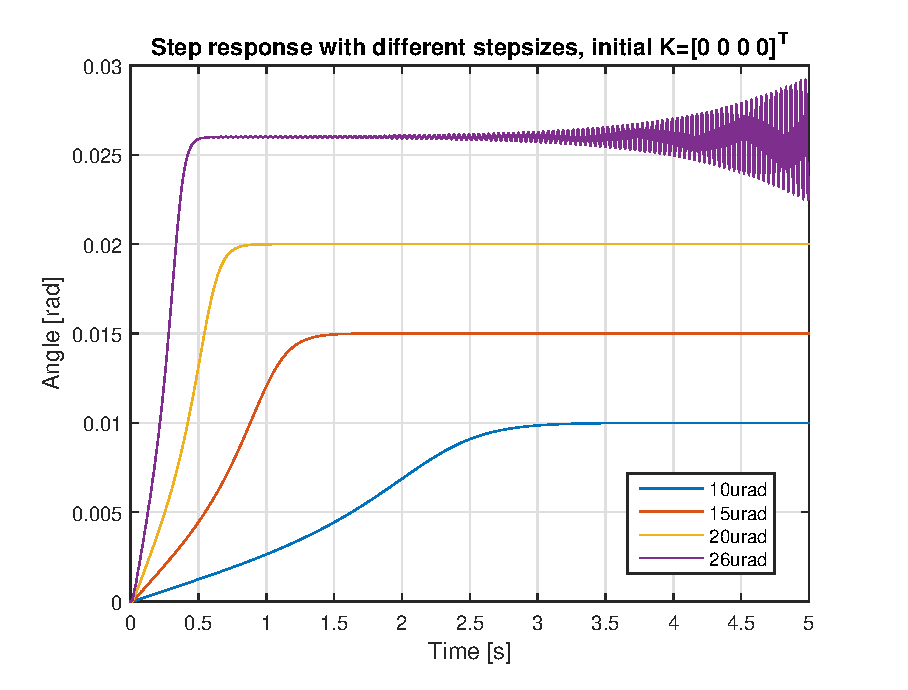
\includegraphics[width=0.7\textwidth]{fig/matlab/stepresponse.eps}
  \caption{\label{fig:step_adaptive} Step responses to step sizes of 10, 15, 20 and 26 mrad.}
\end{figure}

The adaptation process of the control parameters $k_i$, for a step response resulting from a 20mrad step, can be seen in Figure~\ref{fig:adapt_process}. All of the coefficients have converged within 1 second.

\begin{figure}[h!]
  \centering
  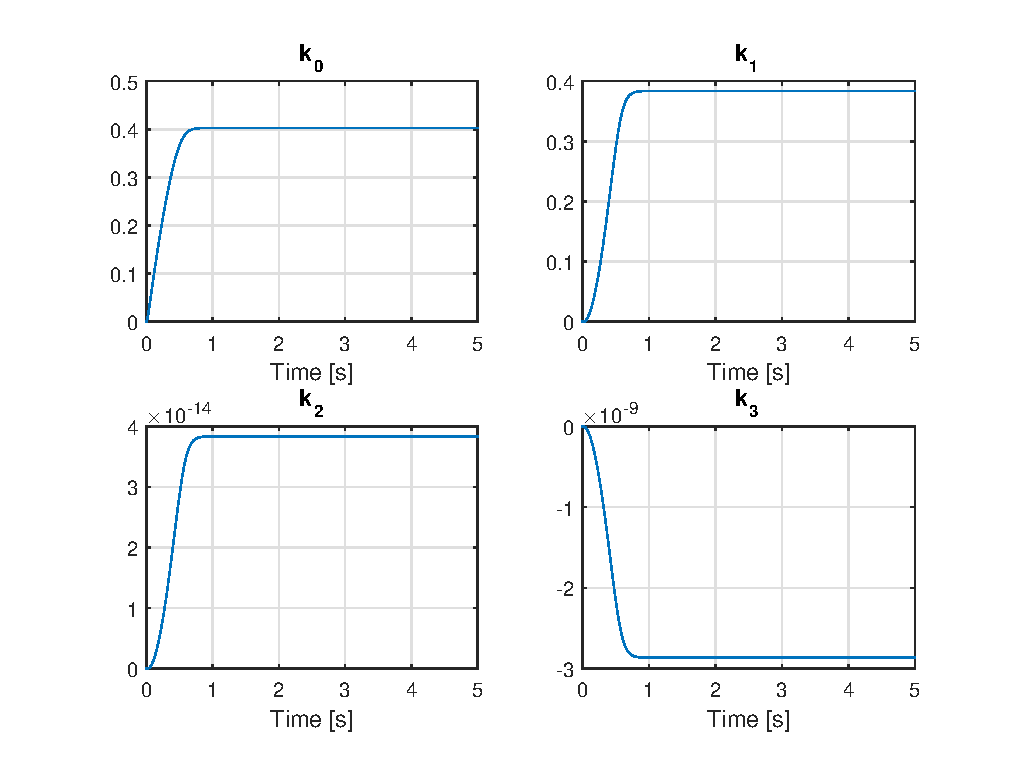
\includegraphics[width=1\textwidth]{fig/matlab/k.eps}
  \caption{\label{fig:adapt_process} Adaptation process of control parameters $k_i$ with a 20 mrad step.}
\end{figure}

To illustrate the adaptation process better, a periodic response is depicted in Figure~\ref{fig:periodic_resp}, here it is clear that after the adaptation process is finished the controller performs better for the second and third period. One can see that the adaptation process is slower for the periodic response corresponding to the amplitude of \unit{10}{\milli\radian}, hence the lower the step, the longer the adaptation time. The present controller performs well for all amplitudes.

\begin{figure}[h!]
  \centering
  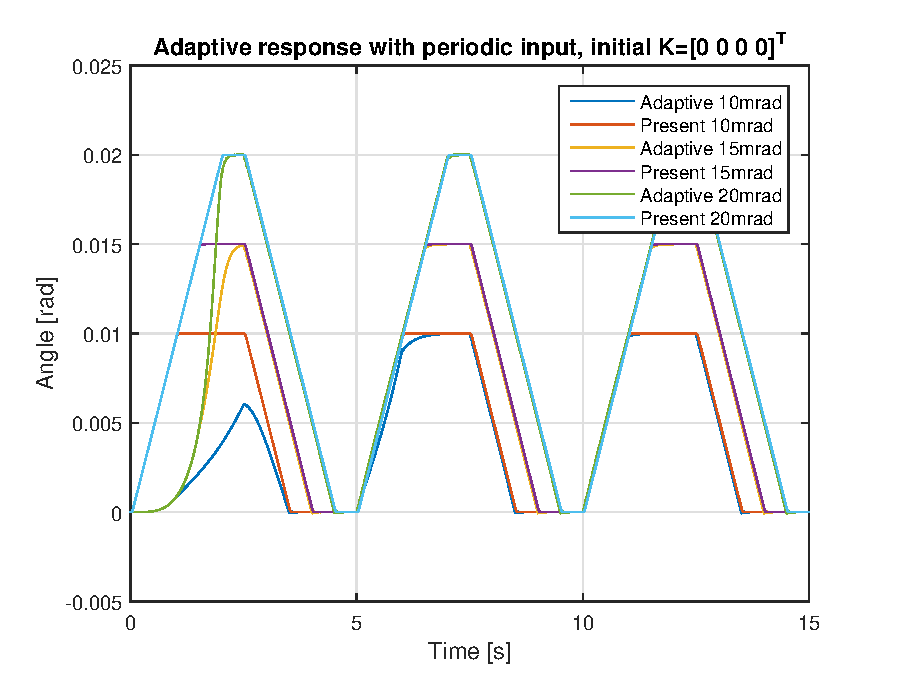
\includegraphics[width=0.7\textwidth]{fig/matlab/periodicresponse.eps}
  \caption{\label{fig:periodic_resp} Periodic responses for the adaptive and present controller with amplitudes of 10, 15, 20 mrad.}
\end{figure}

The tracking error corresponding to the \emph{Adaptive 20mrad} and \emph{Present 20mrad} in Figure~\ref{fig:periodic_resp} can be seen in Figure~\ref{fig:adapt_trackingerror}. The adaptive controller performs better than the present controller after the adaptation process has finished.
\begin{figure}[h!]
  \centering
  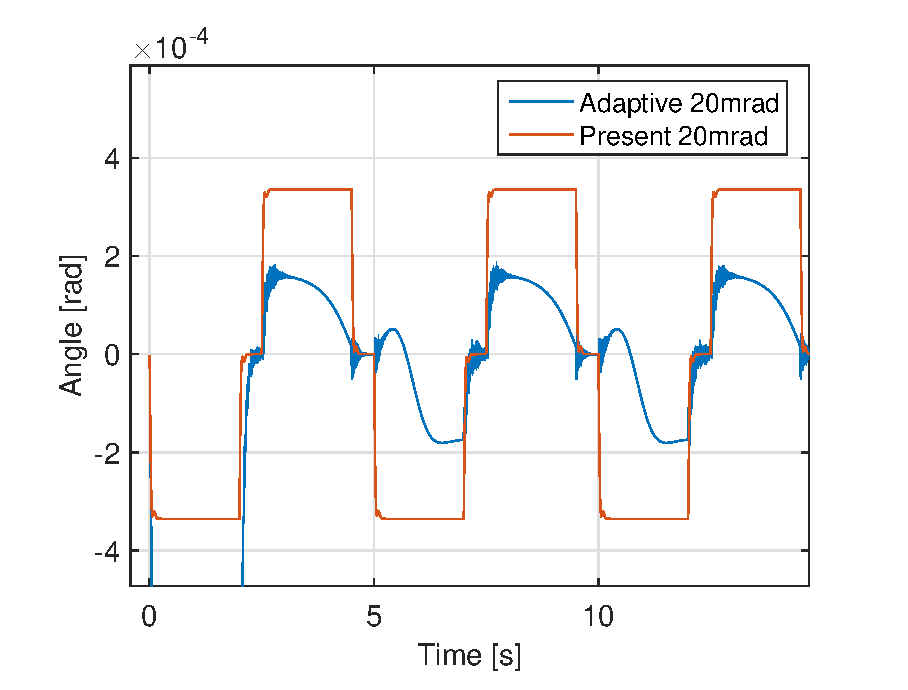
\includegraphics[width=0.7\textwidth]{fig/matlab/trackingerror.eps}
  \caption{\label{fig:adapt_trackingerror} Tracking error (difference between reference and output) for the periodic response from an input signal with an amplitude of 20 mrad.}
\end{figure}

A periodic response with model parameter drift is presented in Figure~\ref{fig:modeldrift}. It shows how the adaptive controller manages to adapt to the change in the system dynamics, while the present controller fails to do so, resulting in an unstable system. The change of the model was performed over 2 seconds, resulting in a movement of the first resonance peak, from 38 Hz to 66 Hz in frequency and from 30.1 dB to 23.5 dB in magnitude. Note that the change of the model is relatively big and for a smaller movement of the resonance peak, the present controller could still be sufficient as illustrated in Figure~\ref{fig:modelerror}.
\begin{figure}[h!]
  \centering %crop: left bottom right top
  \subfloat[][\label{fig:modeldriftresponse}Periodic response with model parameter drift.]{
  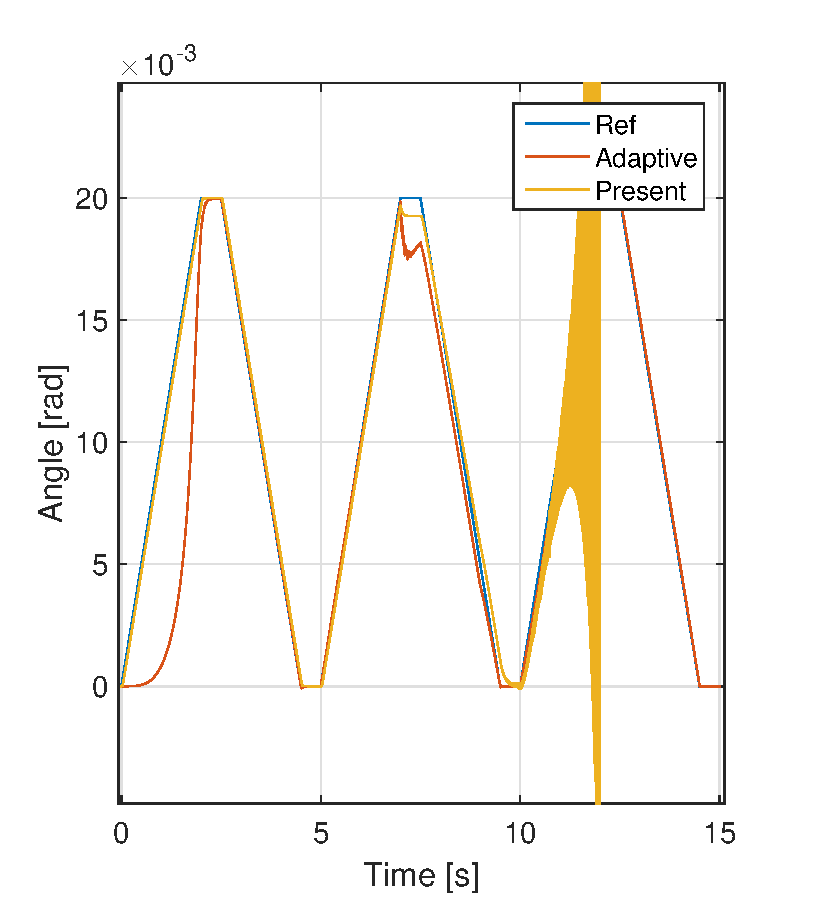
\includegraphics[width=0.46\textwidth, trim=0cm 0cm 1cm 0cm, clip=true]{fig/matlab/driftofmodelparameterover2s.eps}}
  \qquad
  \subfloat[][\label{fig:modeldriftbode}Original model (G) and the resulting model after drift ($G_{mod}$).]{
  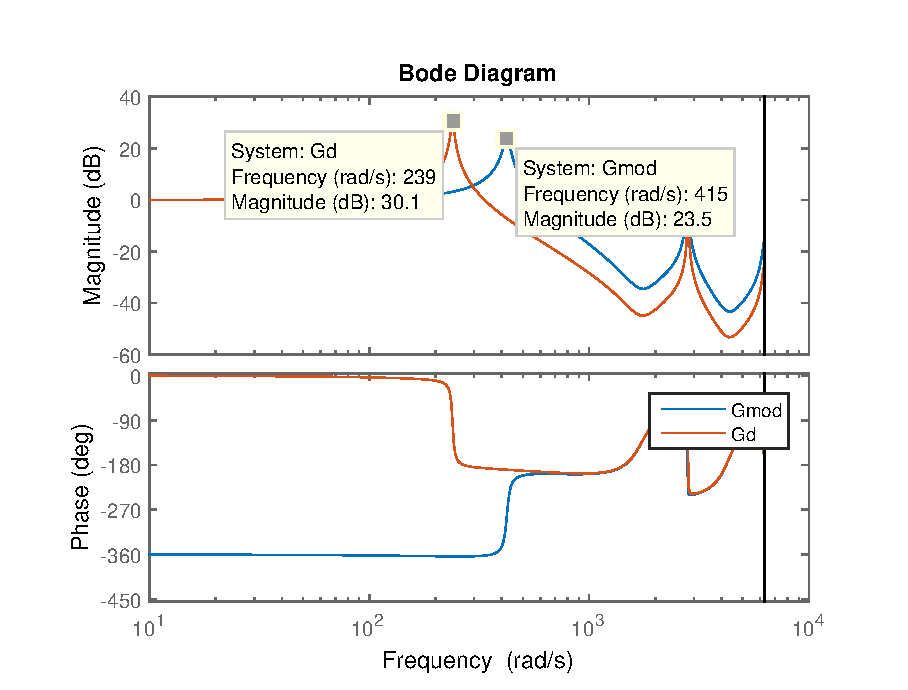
\includegraphics[width=0.46\textwidth, trim=0cm 0cm 0.7cm 0cm, clip=true]{fig/matlab/bode_drift_pole.eps}}
  \caption{\label{fig:modeldrift} Shows the robustness to model changes over time. The model error is increased linearly from $t=7s$ to $t=9s$. The resulting responses is shown in (a) with the model change in (b).}
\end{figure}

\begin{figure}[h!]
  \centering %crop: left bottom right top
  \subfloat[][\label{fig:modelerrorresponse}Periodic response with model parameter drift.]{
  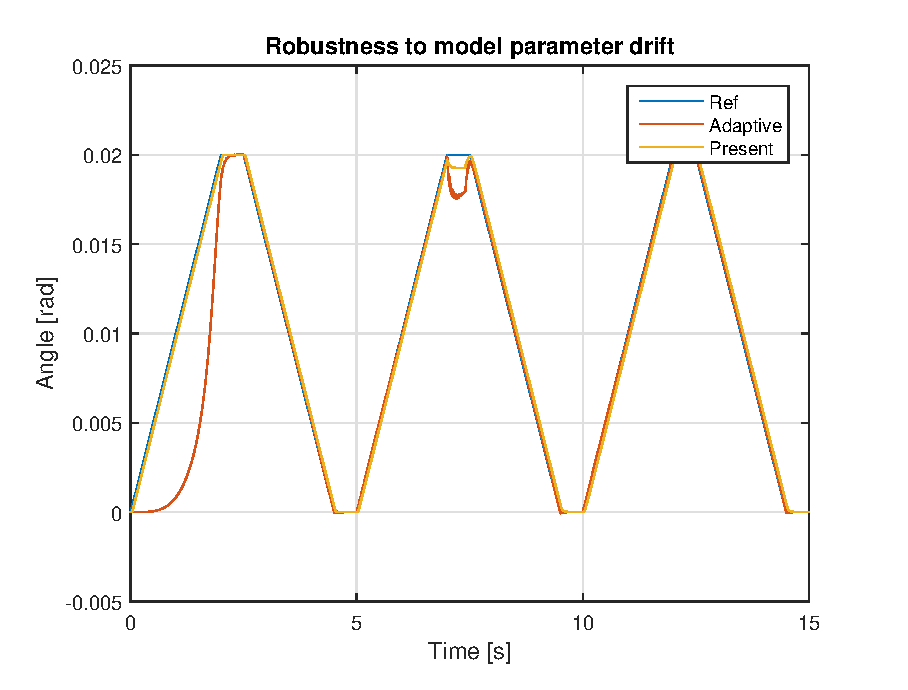
\includegraphics[width=0.46\textwidth, trim=0cm 0cm 1cm 0cm, clip=true]{fig/matlab/modelerrorperiodic.eps}}
  \qquad
  \subfloat[][\label{fig:modelerrorbode}Original model (G) and the resulting model after drift ($G_{mod}$).]{
  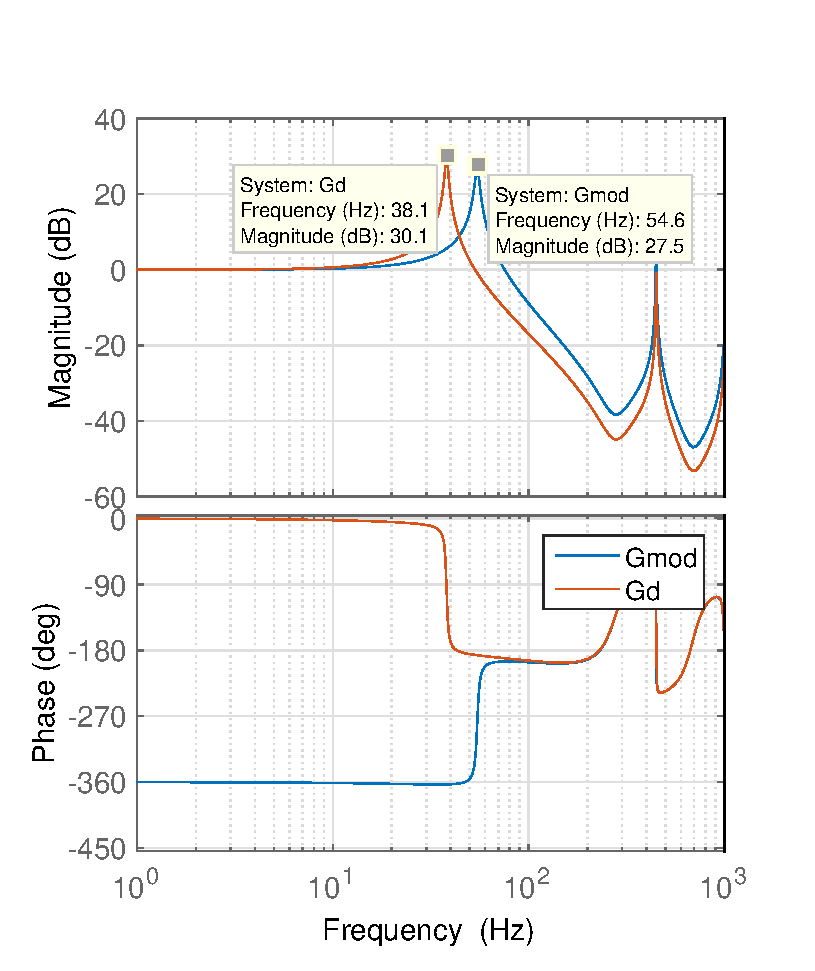
\includegraphics[width=0.46\textwidth, trim=0cm 0cm 0.7cm 0cm, clip=true]{fig/matlab/bode_modelerror_pole.eps}}
  \caption{\label{fig:modelerror}Shows the robustness to model changes over time. The model error is increased linearly from $t=5s$ to $t=7s$. The resulting responses is shown in (a) with the model change in (b).}
\end{figure}

In the case in Figure~\ref{fig:modelerror} the resonance peak is only moved 6.5 Hz and the present controller is sufficient to suppresses the disturbance. It even does it more efficiently than the adaptive controller. Even though the adaptive is slower than the present controller it still produces a smaller tracking error after the adaption process is over, see Figure~\ref{fig:modelerror_trackingerror} Note that the change in the model is equivalent to the change between 0V and 6.5V presented in Figure~\ref{fig:different_angles}.

\begin{figure}[h!]
  \centering
  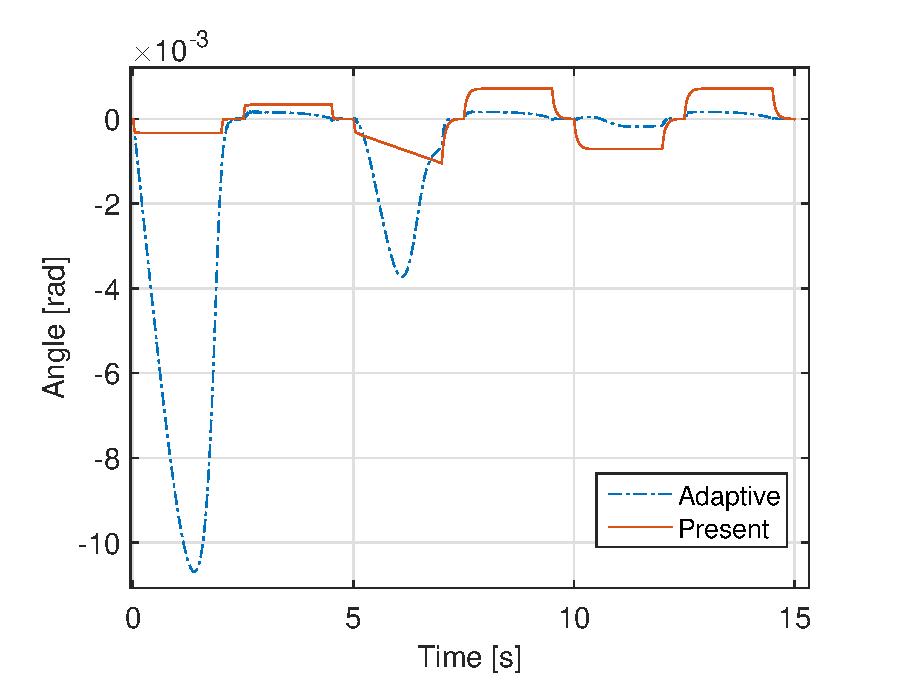
\includegraphics[width=0.7\textwidth]{fig/matlab/modelerrorperiodic_trackingerror.eps}
  \caption{\label{fig:modelerror_trackingerror} Tracking error for the periodic response with a model error drift from $t=5s$ to $t=7s$.}
\end{figure}

Figure~\ref{fig:distrejection} and \ref{fig:distmeasrejection} shows the disturbance rejection capability to a disturbance on the input and output, receptively. In Figure~\ref{fig:distrejection} a small impulse was added to the input to see if the controllers would attenuate it sufficiently. The adaptive controller performed worse than the present controller both with and without pre-filter. The present controller managed to attenuated the highest peak of the impulse by 1.5 times more than the adaptive. The settling time was also approximately 3 times worse for the adaptive controllers. In Figure~\ref{fig:distmeasrejection} the impulse was instead added to the measured signal. Even in this case the present controller was superior, attenuating the highest peak of the impulse by 3 times more than the adaptive controller.

\begin{figure}[h!]
  \centering %crop: left bottom right top
  \subfloat[][\label{fig:dist}Step response]{
  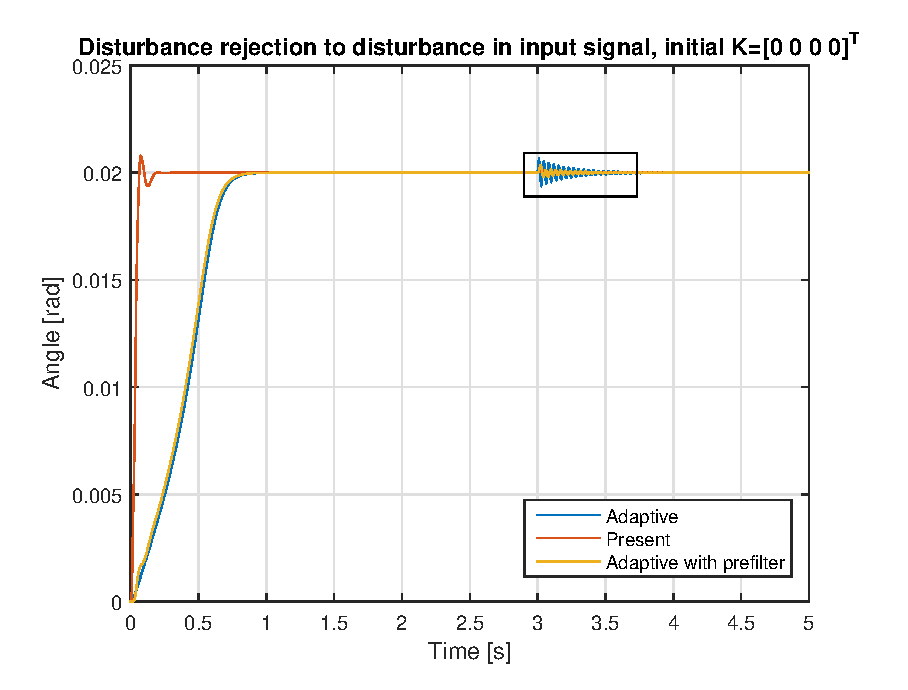
\includegraphics[width=0.46\textwidth, trim=0cm 0cm 1cm 0.8cm, clip=true]{fig/matlab/distrejection.eps}}
  \qquad
  \subfloat[][\label{fig:distzoom}Zoom in on disturbance]{
  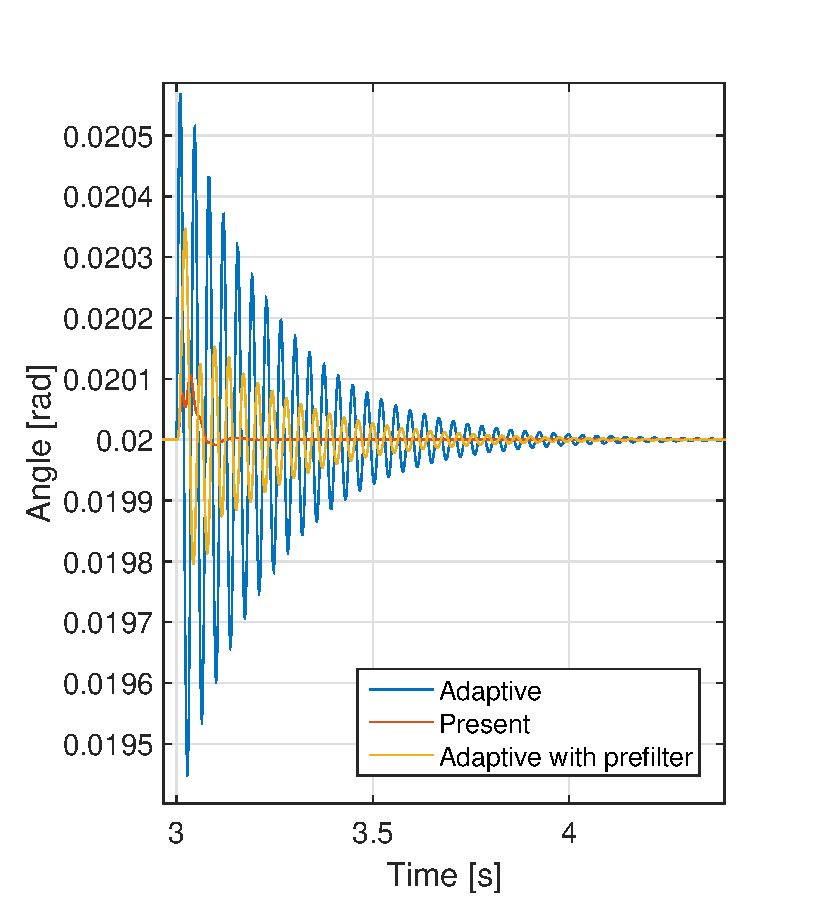
\includegraphics[width=0.46\textwidth, trim=0cm 0cm 1cm 0.8cm, clip=true]{fig/matlab/distrejection_zoom.eps}}
  \caption{\label{fig:distrejection} Shows how well the controller attenuates a disturbance impulse (amplitude of $5.1 \times 10^{-3}$) added to the input signal at $t=3s$. The whole step response is shown in (a) with a zoom in on the disturbance in (b).}
\end{figure}
\begin{figure}[h!]
  \centering %crop: left bottom right top
  \subfloat[][\label{fig:distmeas}Step response]{
  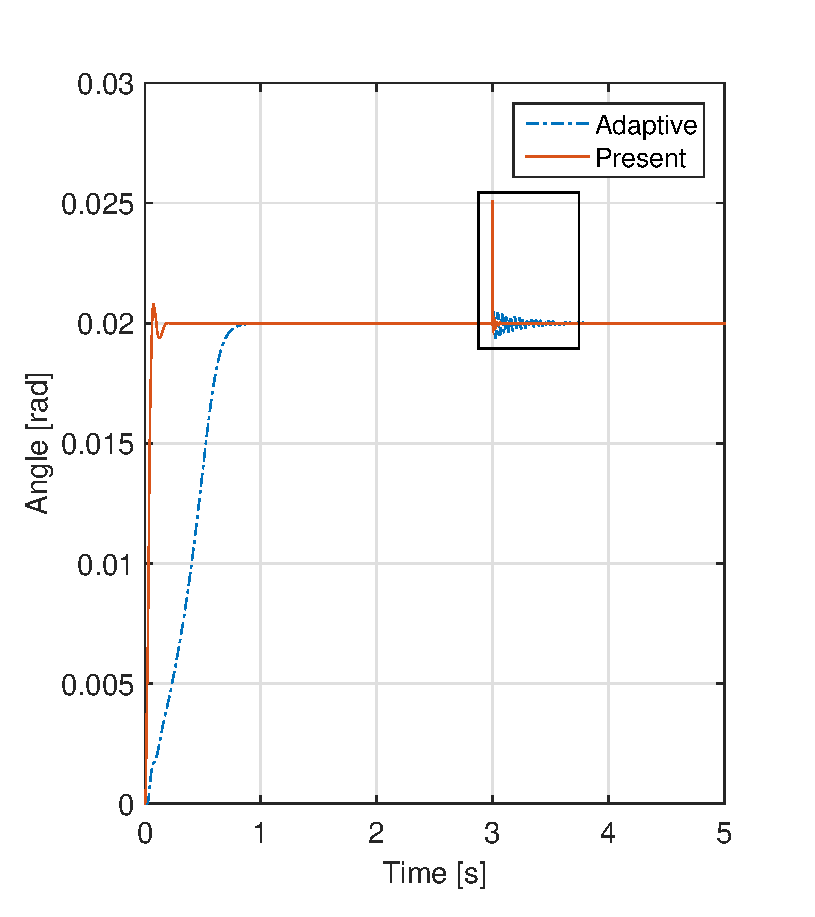
\includegraphics[width=0.46\textwidth, trim=0cm 0cm 1cm 0.8cm, clip=true]{fig/matlab/distrejection_meas.eps}}
  \qquad
  \subfloat[][\label{fig:distmeaszoom}Zoom in on disturbance]{
  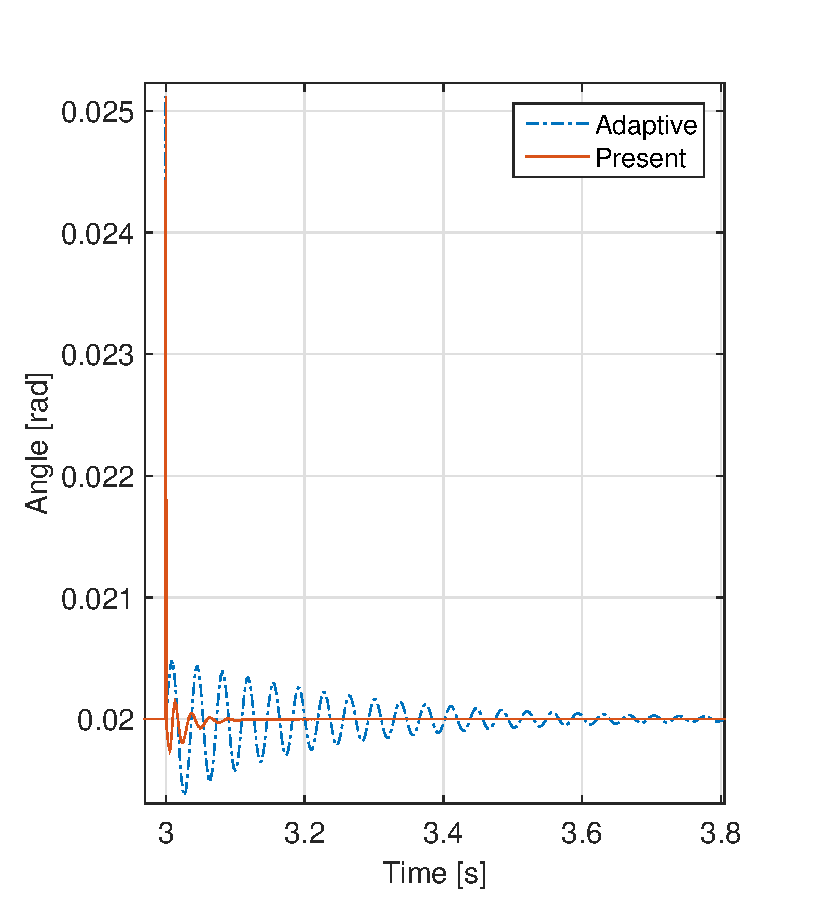
\includegraphics[width=0.46\textwidth, trim=0cm 0cm 1cm 0.8cm, clip=true]{fig/matlab/distrejection_meas_zoom.eps}}
  \caption{\label{fig:distmeasrejection} Disturbance rejection to impulses (amplitude of $5.1 \times 10^{-3}$) added to the measured signal at $t=3s$. The step response is shown in (a)  with a zoom in on the disturbance in (b).}
\end{figure}

\newpage
\subsection{Integral Resonance Control}
The \abbrIRC design procedure presented in \ref{sec:irc} was carried out in continues time, but each block in the scheme was individually discretized for the sake of comparison with the present controller. The continues time system of \eqref{eq:tf} consist of a system with 7 poles and 6 zeros. A negative feedforward would therefore introduce another zero and depending on the gain placing the zeros in a desired position. As seen in the pole-zero plot comparison in Figure~\ref{fig:negfeedpzmap}, a feedforward of $D_f=-1.2$ was sufficient to introduce one zero and place it and its complex conjugate below the first resonance frequency. This and the zero-pole interlacing for the higher order modes can be seen in Figure~\ref{fig:pzafter}, where the zoom-in shows the complex conjugate zeros below the first resonance mode.

\begin{figure}[h!]
  \centering %crop: left bottom right top
  \subfloat[][\label{fig:pzbefore}Origianl system]{
  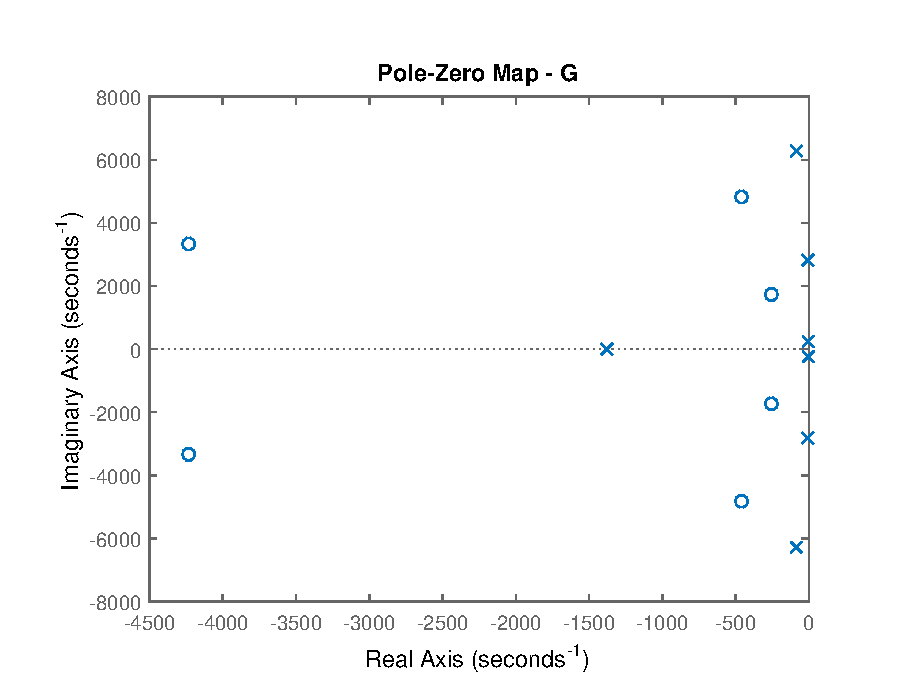
\includegraphics[width=0.46\textwidth, trim=0cm 0cm 1cm 0cm, clip=true]{fig/matlab/pzbefore.eps}}
  \qquad
  \subfloat[][\label{fig:pzafter}After feedforward]{
  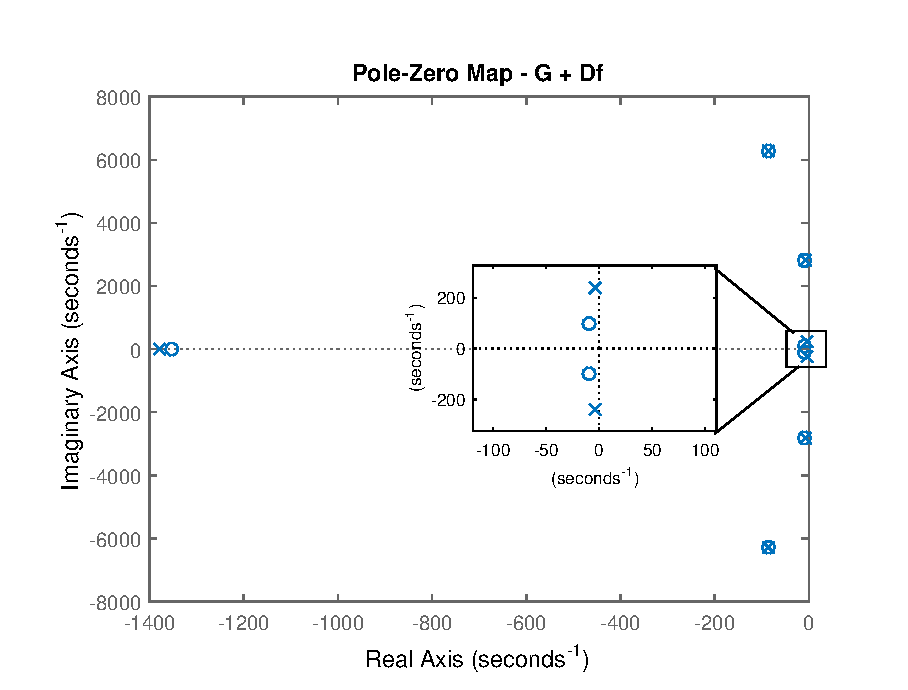
\includegraphics[width=0.46\textwidth, trim=0cm 0cm 1cm 0cm, clip=true]{fig/matlab/pzafter.eps}}
  \caption{\label{fig:negfeedpzmap} Comparison of pole-zero plot before and after adding the negative feedforward. After adding the feedforward to the system which poles and zeros are shown in (a) , the zeros and poles are interlacing as seen in (b).}
\end{figure}

The corresponding bode plot can be seen in Figure~\ref{fig:bodeafterfeedf}, showing the complex conjugate pair of zeros as a dip before the first resonance peak.

\begin{figure}[h!]
  \centering
  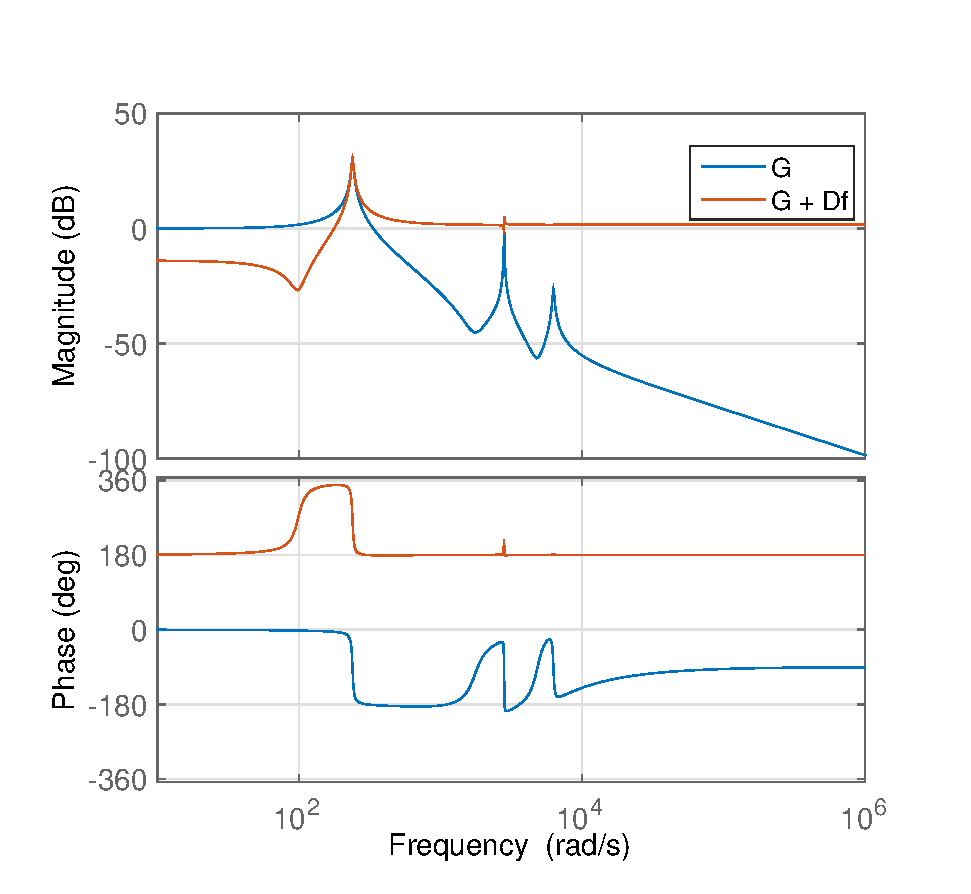
\includegraphics[width=0.7\textwidth]{fig/matlab/bodeafterfeedf.eps}
  \caption{\label{fig:bodeafterfeedf} Bode plot of the system before and after the addition of the negative feedforward.}
\end{figure}

The integral controller $C=\frac{-k}{s}$ was added according to Section~\ref{sec:irc} and a gain of $k=314$ was found to maximize the damping, by using the root locus technique.
The open and closed loop system of the \abbrIRC damping loop depicted in Figure~\ref{fig:irc} is shown in Figure~\ref{fig:bodedamped}. It is clear that the integral controller damps out the first resonance peak efficiently in closed loop.

\begin{figure}[h!]
  \centering
  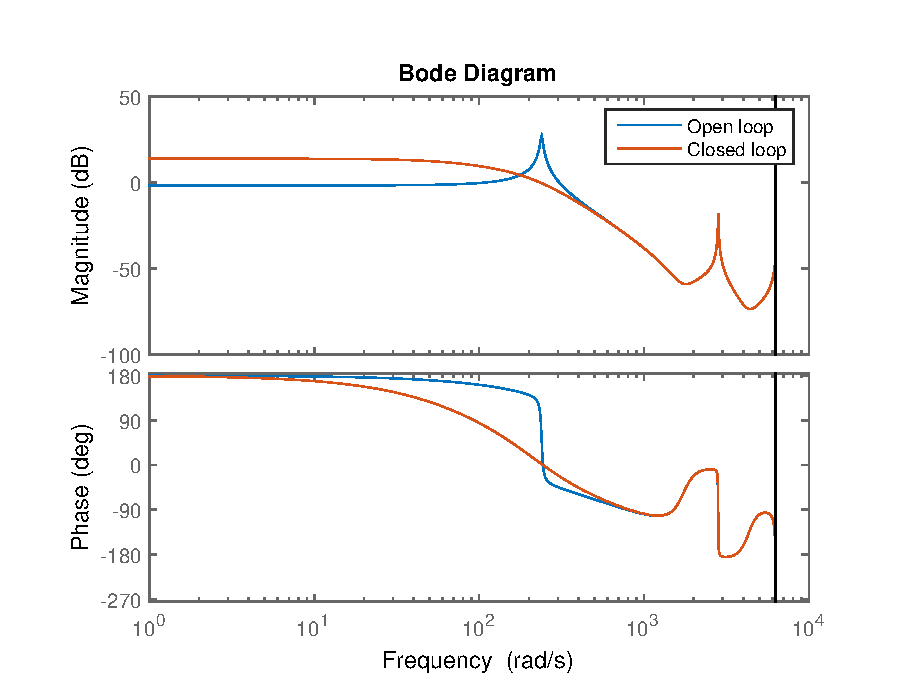
\includegraphics[width=0.7\textwidth]{fig/matlab/bodedamped.eps}
  \caption{\label{fig:bodedamped} Open and closed loop of the IRC damping loop.}
\end{figure}

Finally, the damped system was enclosed in an outer loop with a second controller $C_1$ for reference tracking capability. $C_1$ was designed to be robust to model errors i.e. keep the sensitivity function $G_{dy}$, stated in \eqref{eq:Gyd}, low for the frequencies that the model changes with, (d and y in $G_{dy}$ can be found in the block scheme in Figure~\ref{fig:irc_int}). It was also designed to attenuate higher order resonances using an inclusion of a notch filter.  $C_1$ was designed in Matlab's SISO-Tool and is presented in \eqref{eq:C_1}.

\begin{equation}
  \label{eq:Gyd}
  G_{yd} = \frac{1}{1 + C_2G(1 + C_1)}
\end{equation}

\begin{equation}
  \label{eq:C_1}
  C_1 = \frac{-13.54 z^5 + 40.92 z^4 - 57.47 z^3 + 55.89 z^2 - 35.87 z + 10.05}{z^5 - 1.65 z^4 + 0.80 z^3 - 0.16 z^2 + 0.014 z - 0.00042}
\end{equation}

The resulting closed loop system and the sensitivity function is shown in Figure~\ref{fig:irc_totalclosed} and \ref{fig:sensitivity_irc}, respectively. The plots show that the use of the \abbrIRC has increased the closed loop bandwidth from 11 Hz to 73 Hz, corresponding to an increase of 6.5 times the present closed loop bandwidth.

\begin{figure}[h!]
  \centering
  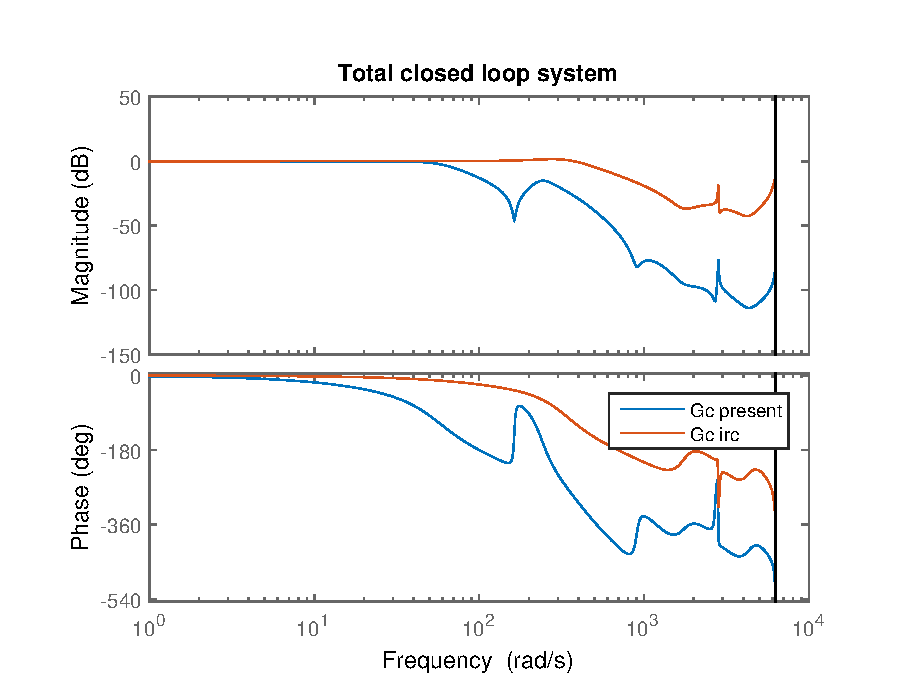
\includegraphics[width=0.7\textwidth]{fig/matlab/totalclosedloop.eps}
  \caption{\label{fig:irc_totalclosed} Closed loop system of the \abbrIRC and the present approach}
\end{figure}

The \abbrIRC sensitivity function also shows that the \abbrIRC scheme attenuates model disturbances better in the low frequency range and in the region within 24-64 Hz.

\begin{figure}[h!]
  \centering
  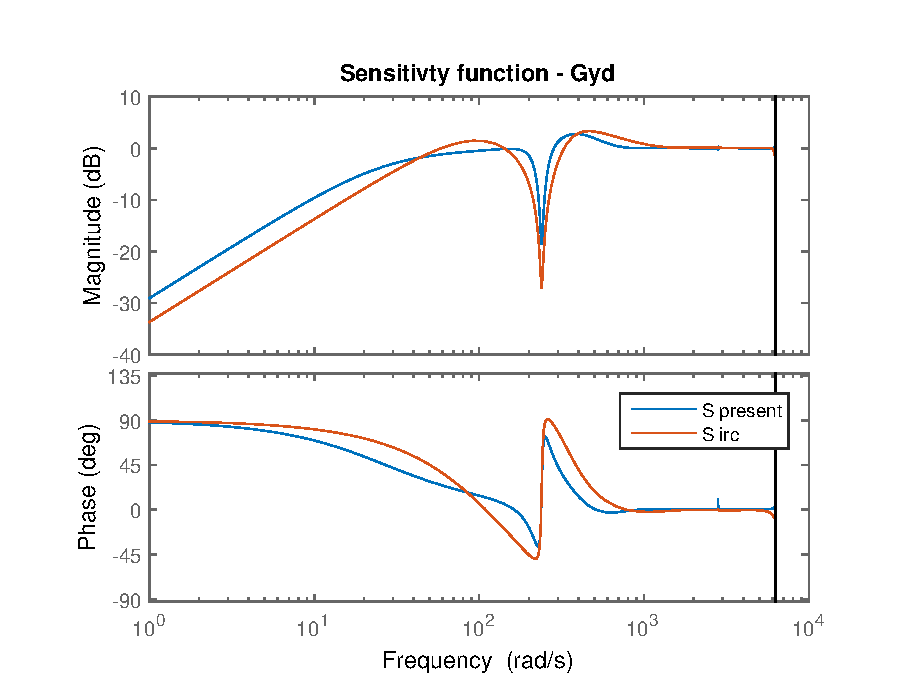
\includegraphics[width=0.7\textwidth]{fig/matlab/sensitivity_irc.eps}
  \caption{\label{fig:sensitivity_irc}Sensitivity function ($G_{dy}$) of the \abbrIRC and the present approach}
\end{figure}

The \abbrIRC tracking performance is shown in Figure~\ref{fig:irc_tracking}. One can conclude that neither the present nor the \abbrIRC eliminate the constant ramp tracking error. However the \abbrIRC performs better due to its high bandwidth, see Figure~\ref{fig:irc_periodic} for the response and the tracking error in Figure~\ref{fig:irc_tracking}.

\begin{figure}[h!]
  \centering %crop: left bottom right top
  \subfloat[][\label{fig:irc_periodic}Periodic Response]{
  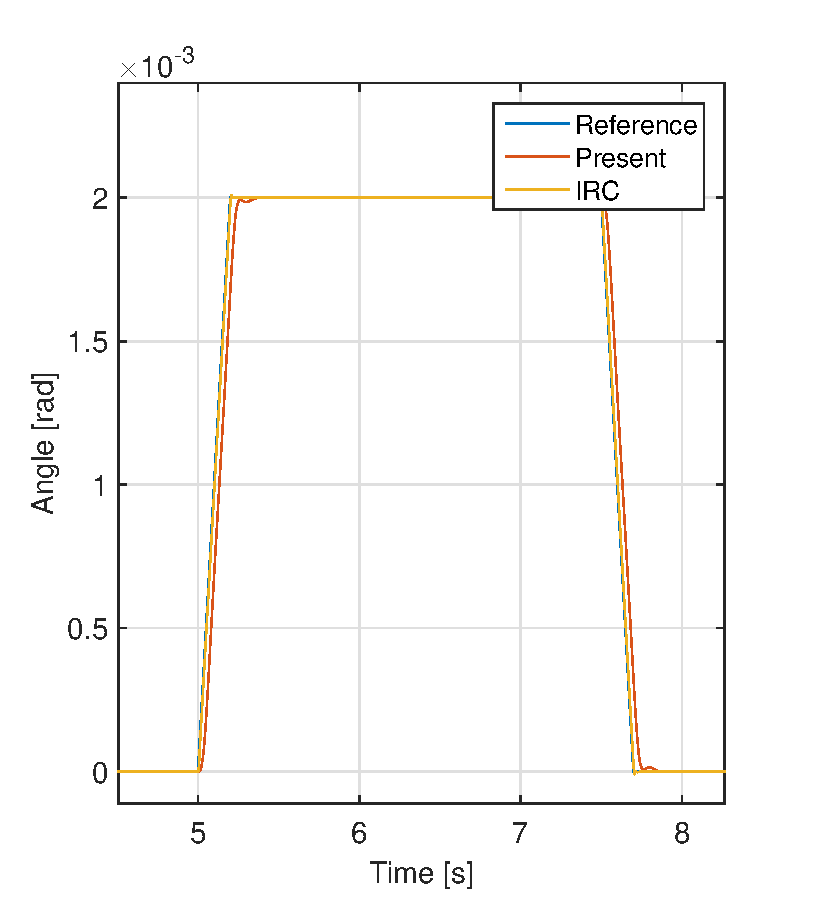
\includegraphics[width=0.46\textwidth, trim=0cm 0cm 1cm 0cm, clip=true]{fig/matlab/irc_periodic.eps}}
  \qquad
  \subfloat[][\label{fig:irc_tracking_error}Tracking error]{
  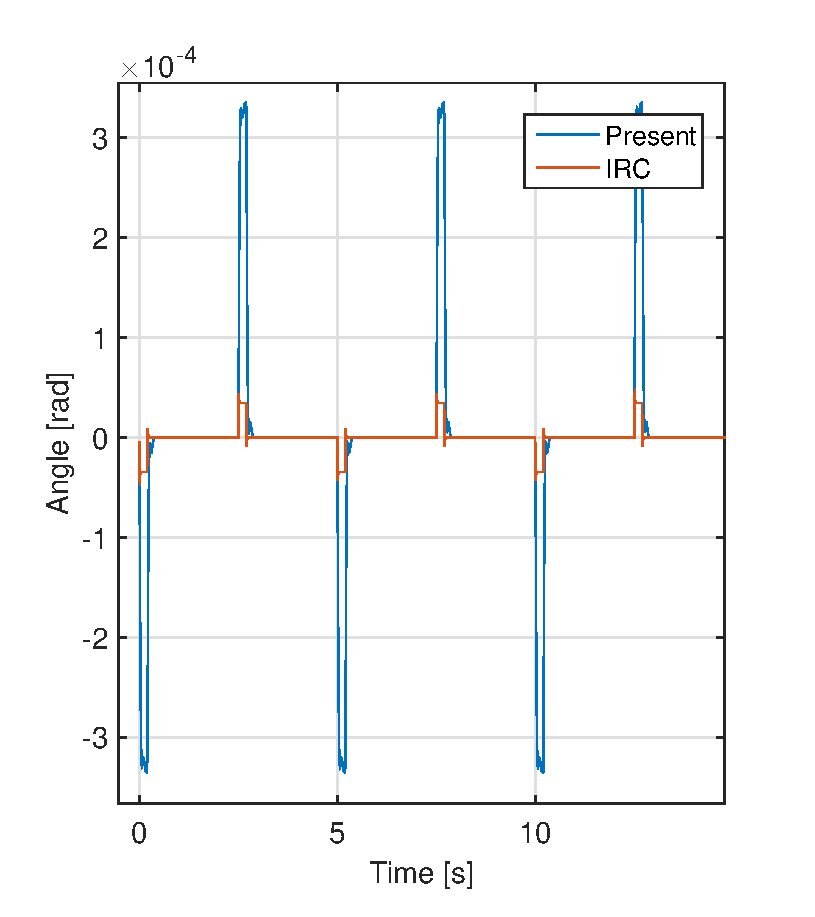
\includegraphics[width=0.46\textwidth, trim=0cm 0cm 1cm 0cm, clip=true]{fig/matlab/irctrackingerror.eps}}
  \caption{\label{fig:irc_tracking} Periodic response of the \abbrIRC and the present controller. A zoom in on one period is shown in (a) while a the tracking error over three periods are shown in (b).}
\end{figure}

The robustness test performed for the adaptive controller was done for the \abbrIRC controller accordingly. Figure~\ref{fig:irc_dist_model} shows the periodic response and its tracking error when the model is changed linearly according to Figure~\ref{fig:modelerrorbode}. The \abbrIRC handles the model drift better than the present controller.

\begin{figure}[h!]
  \centering %crop: left bottom right top
  \subfloat[][\label{fig:irc_dist_model}Periodic response]{
  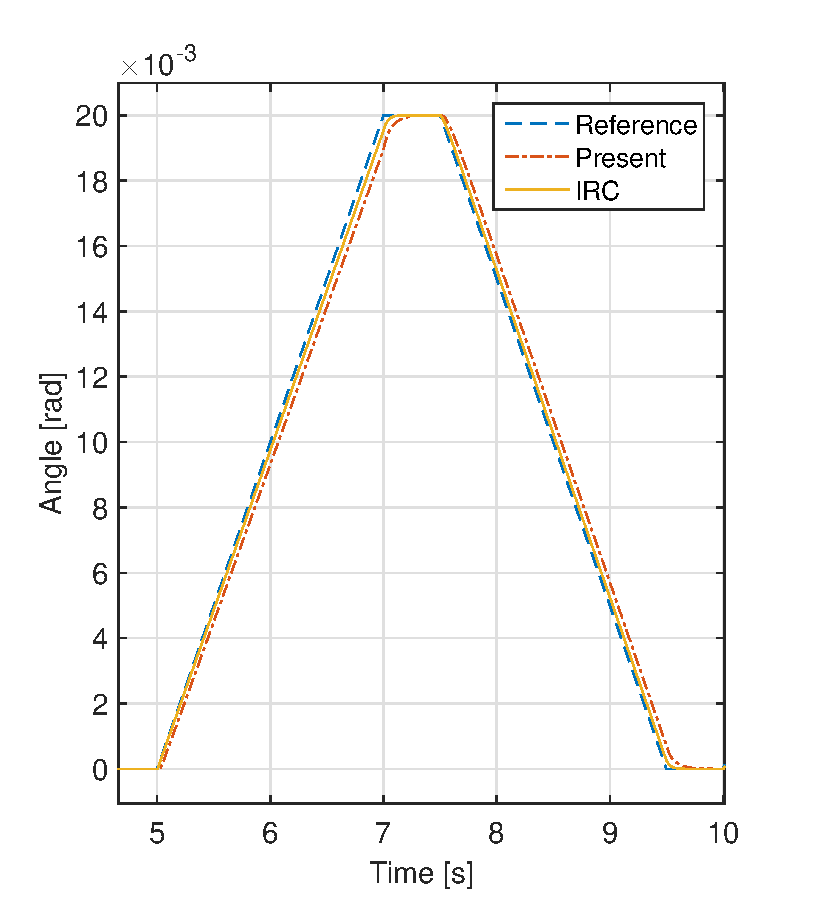
\includegraphics[width=0.46\textwidth, trim=0cm 0cm 1cm 0cm, clip=true]{fig/matlab/irc_periodic_drift.eps}}
  \qquad
  \subfloat[][\label{fig:irc_dist_model_drift}Periodic response with model parameter drift.]{
  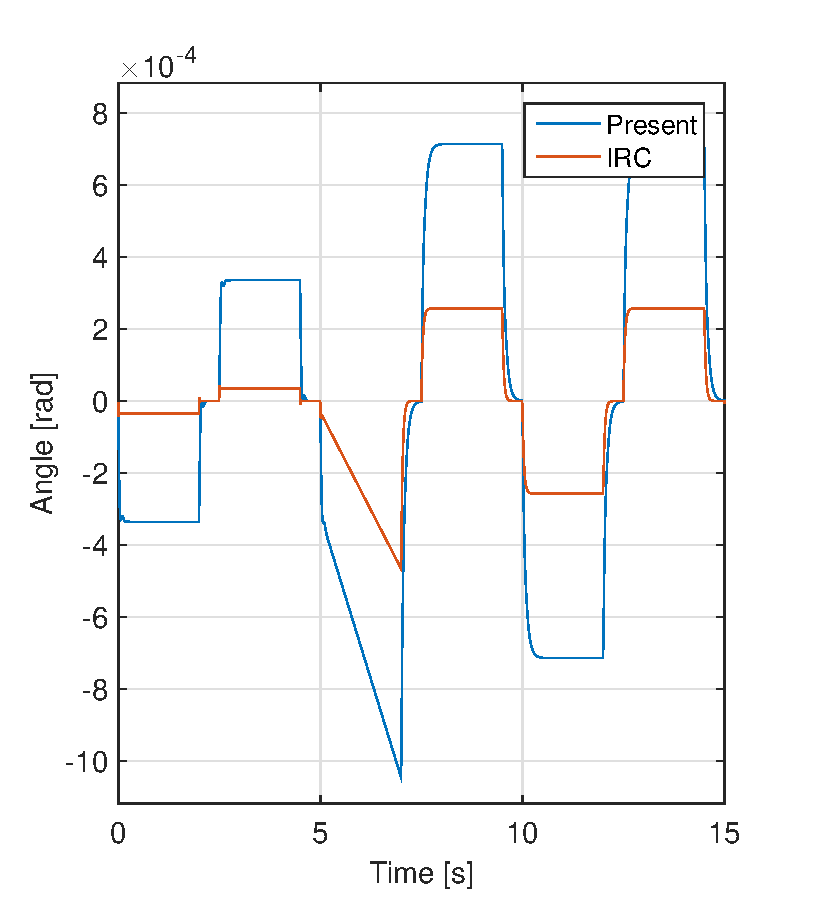
\includegraphics[width=0.46\textwidth, trim=0cm 0cm 1cm 0cm, clip=true]{fig/matlab/irc_periodic_trackingerror.eps}}
  \caption{\label{fig:irc_dist} Shows the robustness to model changes over time. The model error is increased linearly from $t=5s$ to $t=7s$.  A zoom in on one period is shown in (a) while a the tracking error over three periods are shown in (b).}
\end{figure}



The \abbrIRC capability of rejecting disturbances on the input signal is shown in Figure~\ref{fig:irc_dist_input}. As seen in the zoom-in, the \abbrIRC is slightly more damped but has a high frequency ringing in 448Hz, the same frequency as the model's second resonance peak. This ringing is also showing in the present controller but is less dominant.

\begin{figure}[h!]
  \centering %crop: left bottom right top
  \subfloat[][\label{fig:irc_dist_input_step}Step response]{
  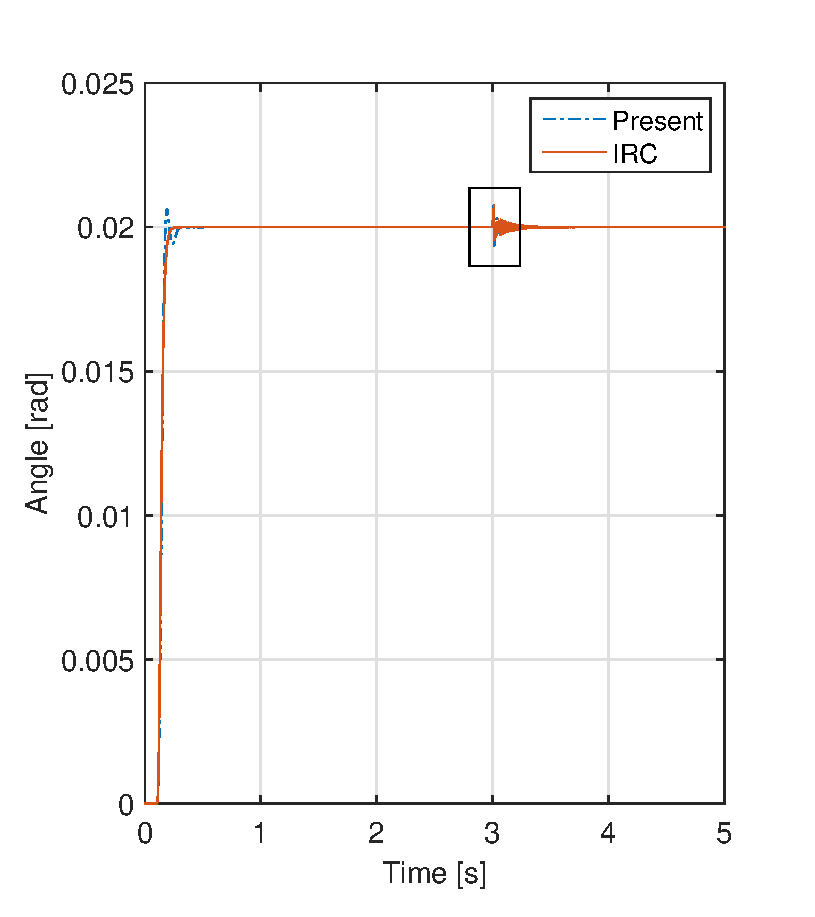
\includegraphics[width=0.46\textwidth, trim=0cm 0cm 1cm 0cm, clip=true]{fig/matlab/irc_dist_input.eps}}
  \qquad
  \subfloat[][\label{fig:irc_dist_input_zoom}Zoom in on disturbance]{
  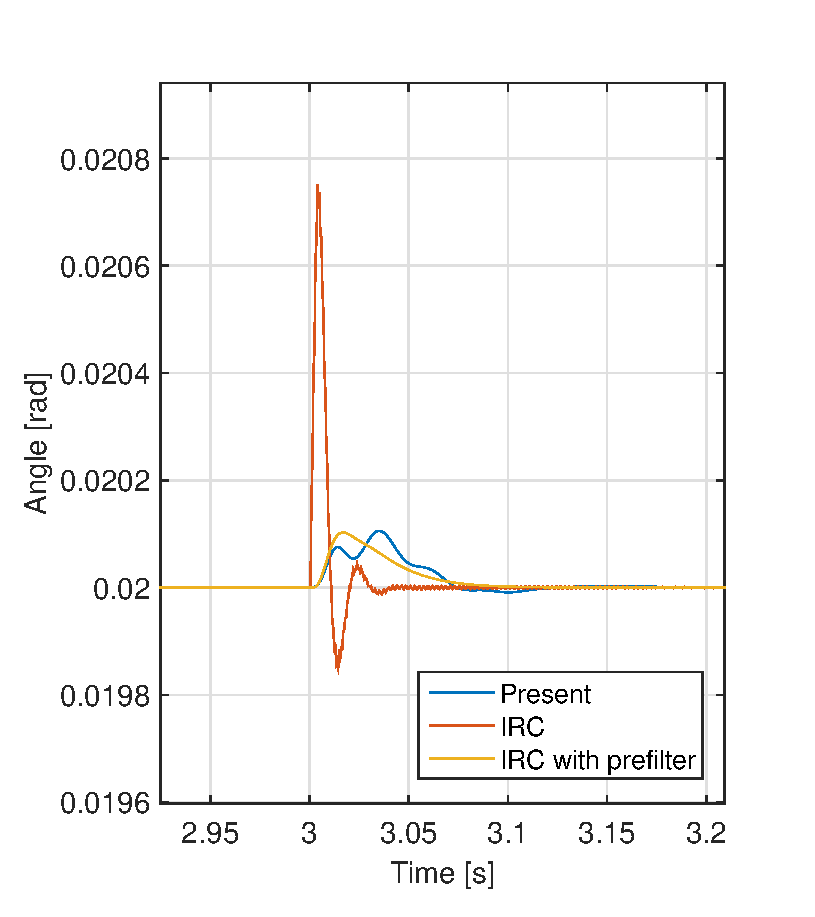
\includegraphics[width=0.46\textwidth, trim=0cm 0cm 1cm 0cm, clip=true]{fig/matlab/irc_dist_input_zoom.eps}}
  \caption{\label{fig:irc_dist_input} Shows how well the controller attenuates a disturbance impulse (amplitude of $5.1 \times 10^{-3}$) added to the input signal at $t=3s$. The whole step response is shown in (a) with a zoom in on the disturbance in (b).}
\end{figure}

The \abbrIRC capability of rejecting disturbances on the output signal is shown in Figure~\ref{fig:irc_dist_output}. Since the impulse is added directly on the output the steps response peaks accordingly at $t=3s$. It is hard to tell from Figure~\ref{fig:irc_dist_output_zoom}, but the peak is visible for both of the control approaches. After the peak, the methods perform similarly, with a slightly higher damping and amplitude for the \abbrIRC oscillations shown in the zoom in.

\begin{figure}[h!]
  \centering %crop: left bottom right top
  \subfloat[][\label{fig:irc_dist_output_step}Step response]{
  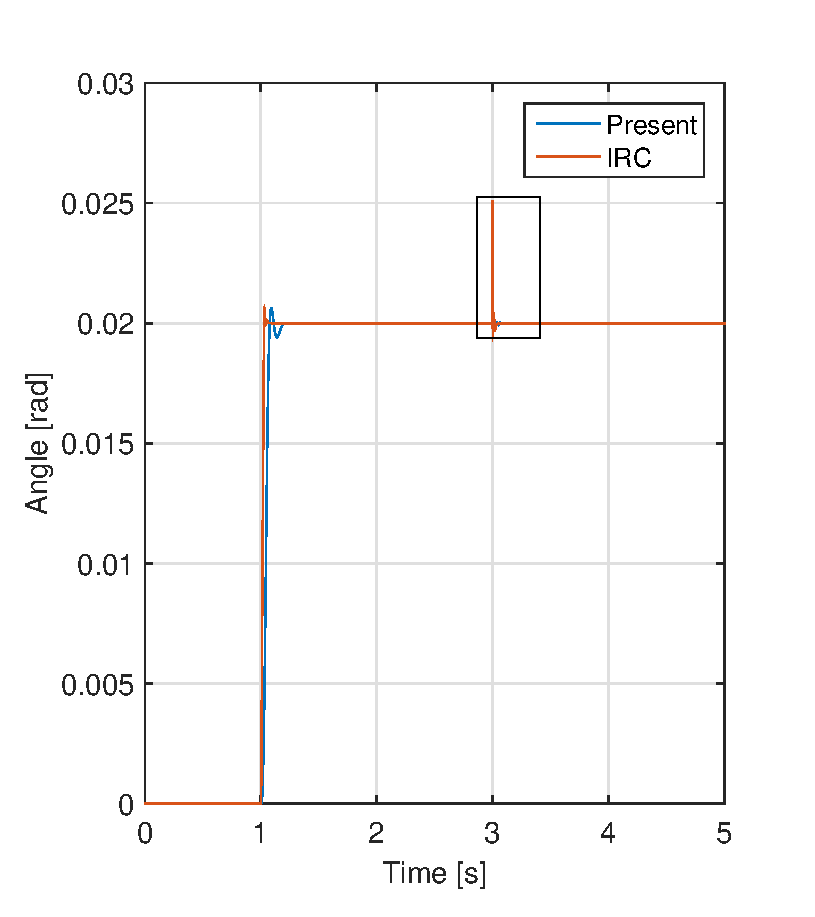
\includegraphics[width=0.46\textwidth, trim=0cm 0cm 1cm 0cm, clip=true]{fig/matlab/distrej_meas.eps}}
  \qquad
  \subfloat[][\label{fig:irc_dist_output_zoom}Zoom in on disturbance]{
  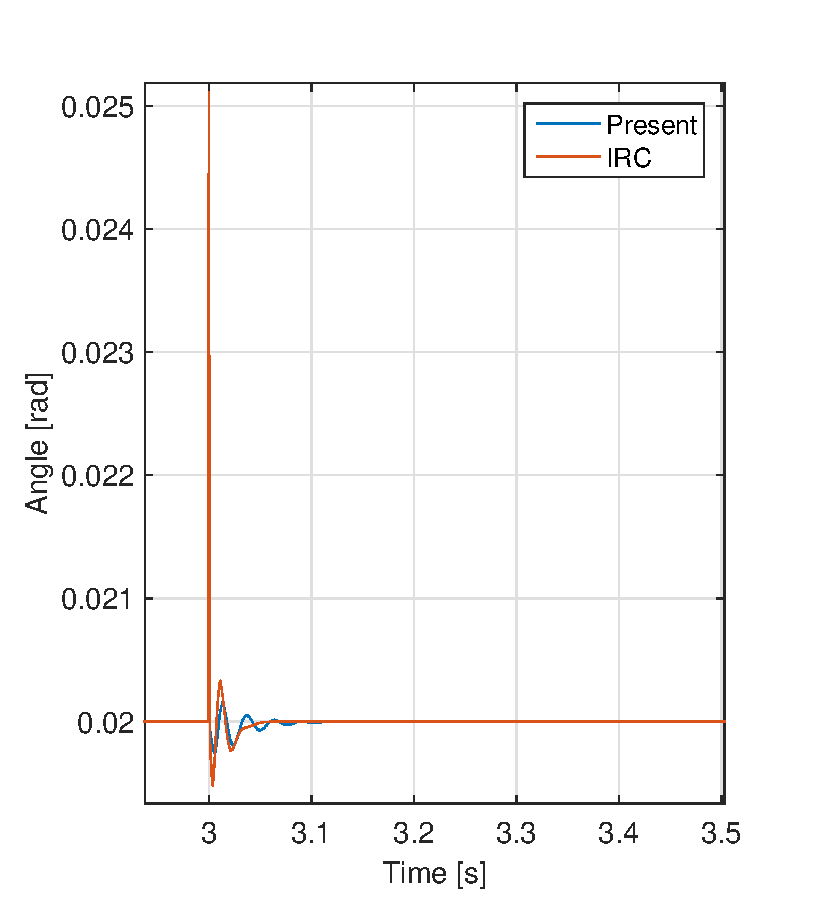
\includegraphics[width=0.46\textwidth, trim=0cm 0cm 1cm 0cm, clip=true]{fig/matlab/distrej_meas_zoom.eps}}
  \caption{\label{fig:irc_dist_output} Shows how well the controller attenuates a disturbance impulse (amplitude of $5.1 \times 10^{-3}$) added to the output signal at $t=3s$. The whole step response is shown in (a) with a zoom in on the disturbance in (b).}
\end{figure}

To further verify the controller capability of handling disturbances with various frequencies, a white noise was added to the input and output signal of the rotational stage ($G$), illustrated in Figure~\ref{fig:irc_int} as $d_i$ and $d_o$, respectively. The \abbrFFT was then performed on the output ($y$) to verify the disturbance rejection for all frequencies, and the result is presented in Figure~\ref{fig:fft_in} and Figure~\ref{fig:fft_out}.

\begin{figure}[h!]
  \centering
  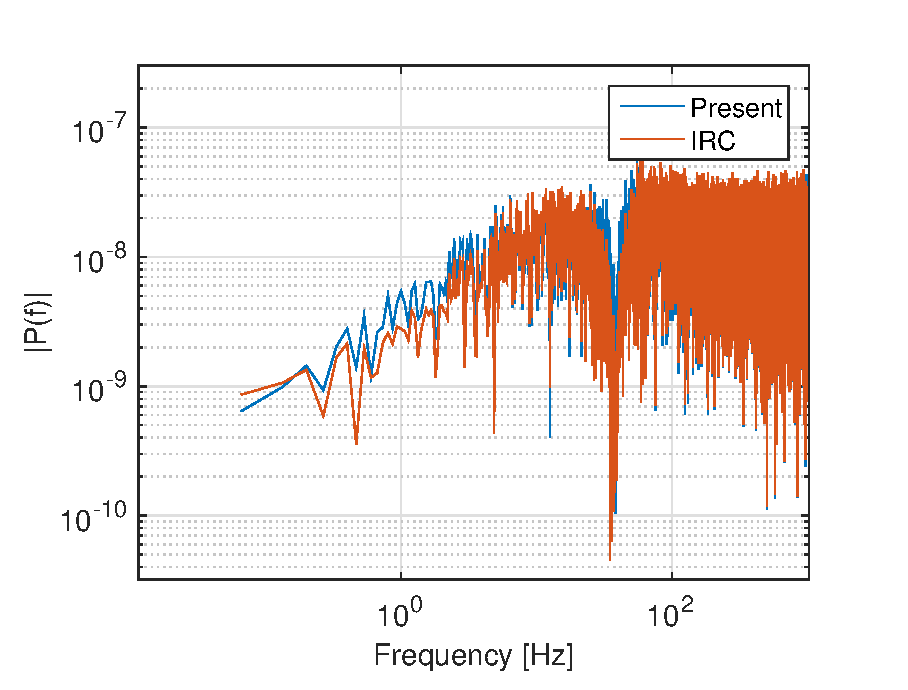
\includegraphics[width=0.7\textwidth]{fig/matlab/whitenoiseoutput.eps}
  \caption{\label{fig:fft_in} The \abbrFFT of the output signal for the \abbrIRC and the present approach, when applying a white noise to the input of G}
\end{figure}

\begin{figure}[h!]
  \centering
  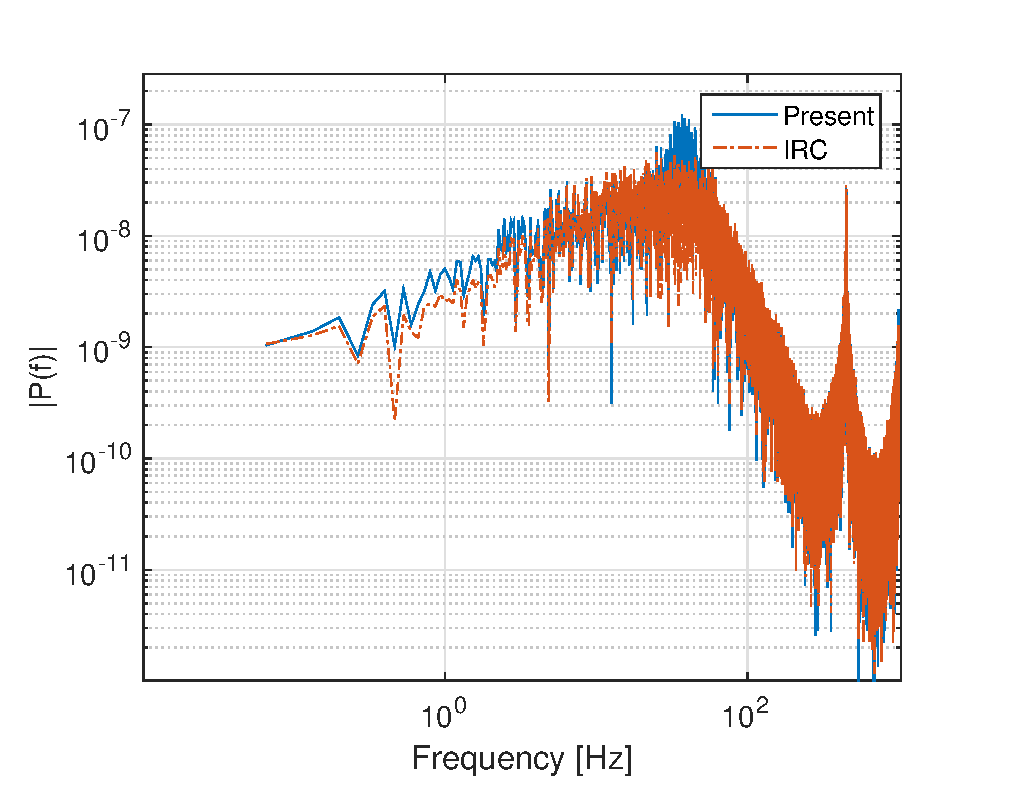
\includegraphics[width=0.7\textwidth]{fig/matlab/whitenoiseinput.eps}
  \caption{\label{fig:fft_out} The \abbrFFT of the output signal for the \abbrIRC and the present approach, when applying a white noise to the output of G}
\end{figure}


The standard deviations for the output signal with the disturbance added to both the output and input for the \abbrIRC and the present approach are summarized in

\begin{table}[h!]
  \centering
  \begin{tabular}{| l | l | l |}
    \hline
    Disturbance applied to: & input & output \\ \hline
      $\sigma_{Present}$ & $6.8097 \times 10^{-7}$ & $1.4336 \times 10^{-6}$ \\
      $\sigma_{IRC}$ & $4.5074 \times 10^{-7}$  & $ 1.4588 \times 10^{-6}$ \\
    \hline
  \end{tabular}
  \caption{\label{tab:std} Standard deviations of the output signal}
\end{table}

Since the \abbrIRC closed loop bandwidth is a lot higher than the present controller, it is expected that the \abbrIRC is more sensitive to measurement noise and to model errors in terms of stability. Both approaches uses a static notch filter to cancel higher order harmonics, which makes the cancellation sensitive for model changes in the higher resonances. Both make it interesting to see how robust the controller are to model changes in the higher frequencies. A disturbance rejection test was performed on the systems showed in Figure~\ref{fig:high_model_error}, where the highest resonance peak has been moved 83Hz and 97Hz, respectively. An impulse was applied to the output and the resulting response is presented in Figure~\ref{fig:model_dist_high_order}. The \abbrIRC is clearly more sensitive to model errors and becomes unstable when the highest resonance peak has moved by 97Hz.

\begin{figure}[h!]
  \centering
  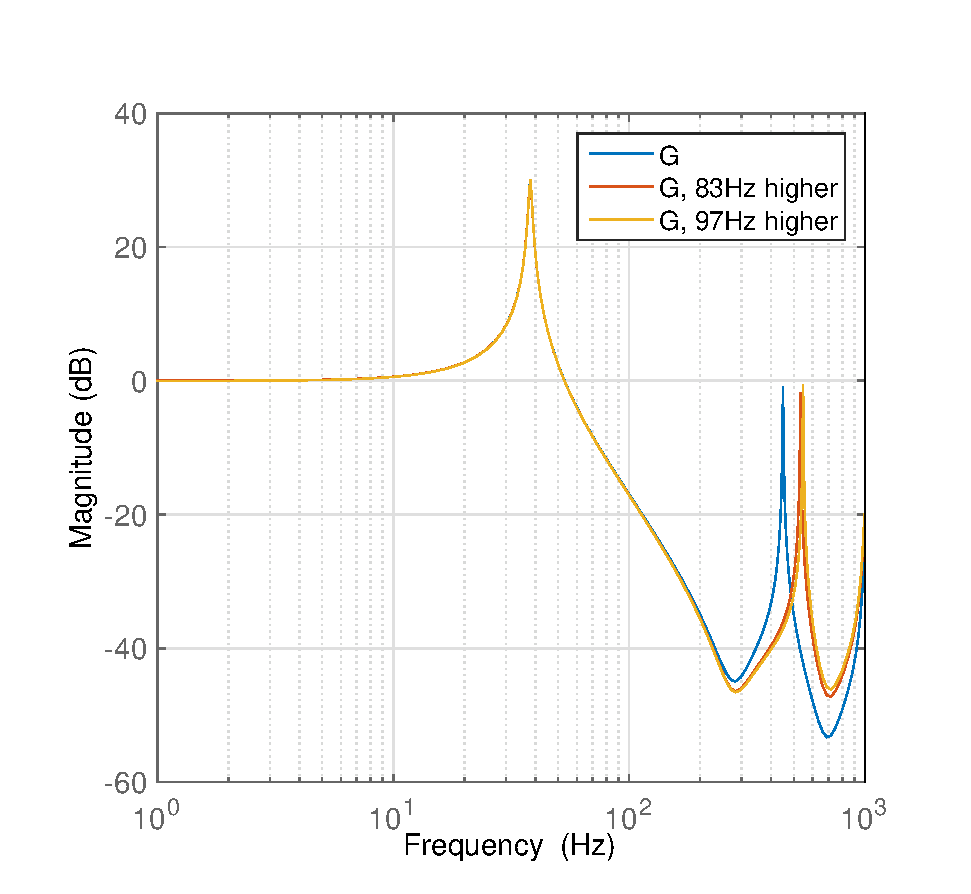
\includegraphics[width=0.7\textwidth]{fig/matlab/bode_high_model_error.eps}
  \caption{\label{fig:high_model_error} The \abbrFFT of the output signal for the \abbrIRC and the present approach, when applying a white noise to the output of G}
\end{figure}


\begin{figure}[h!]
  \centering %crop: left bottom right top
  \subfloat[][\label{fig:model_83}Model change of 83hz]{
  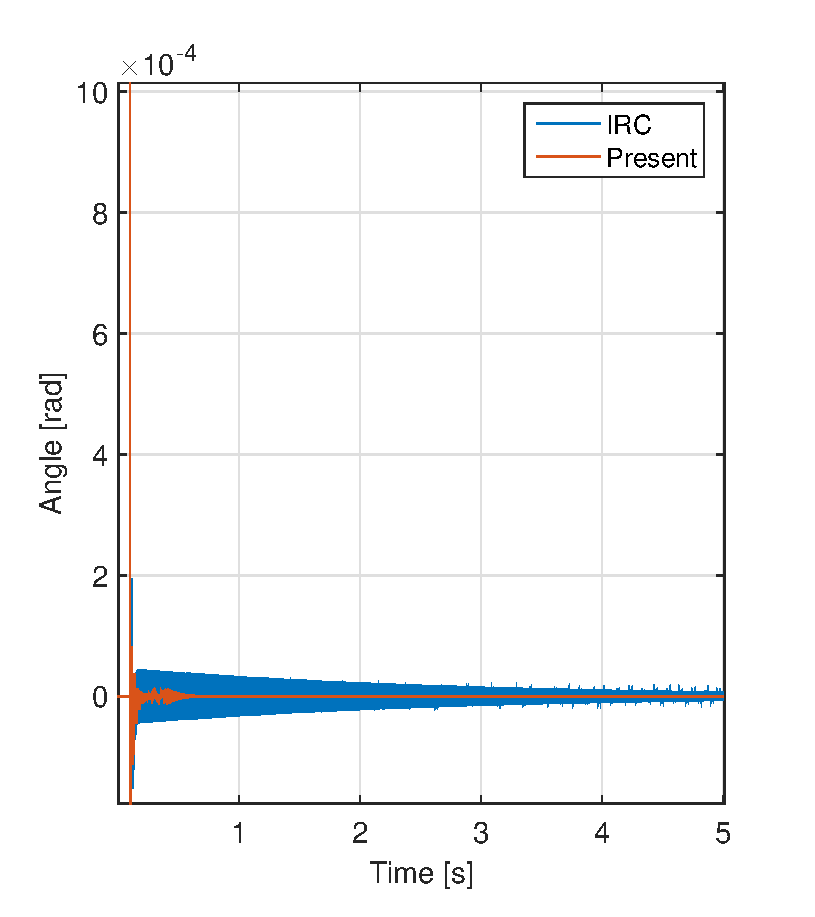
\includegraphics[width=0.46\textwidth, trim=0cm 0cm 1cm 0cm, clip=true]{fig/matlab/model_high_83hz.eps}}
  \qquad
  \subfloat[][\label{fig:model_97}Model change of 97hz]{
  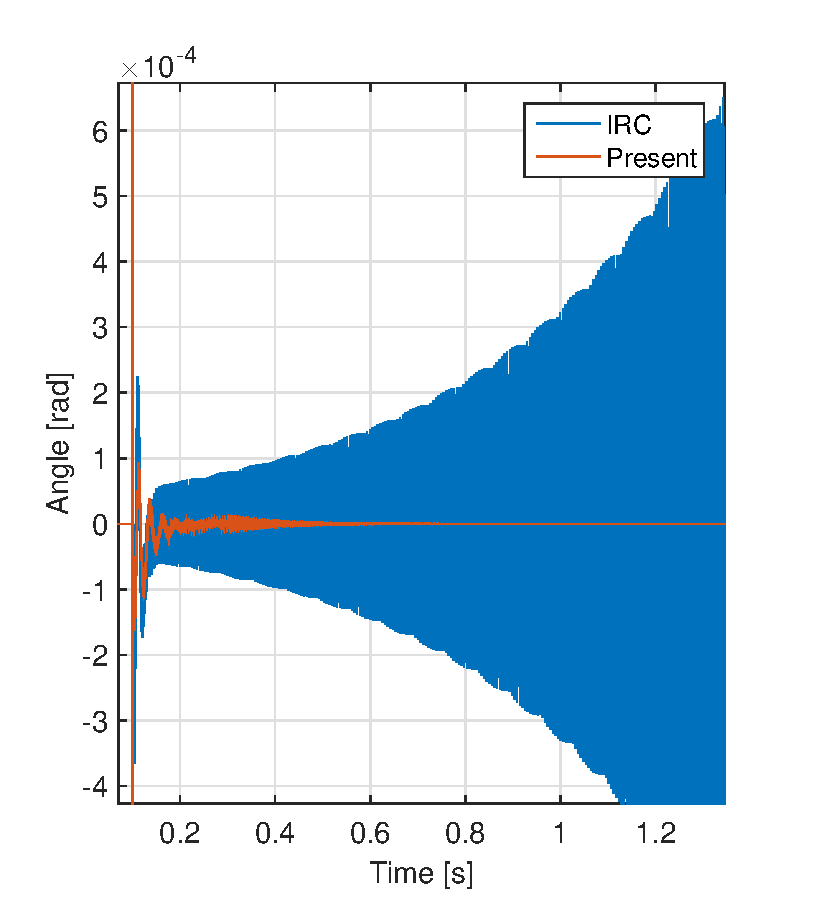
\includegraphics[width=0.46\textwidth, trim=0cm 0cm 1cm 0cm, clip=true]{fig/matlab/model_high_97hz.eps}}
  \caption{\label{fig:model_dist_high_order} Shows how the controller attenuates a disturbance impulse (amplitude of $5.1 \times 10^{-3}$) added to the output signal at $t=0.1s$. The highest resonance peak for the system model G has in (a) been moved by 83Hz and in (b) by 97Hz.}
\end{figure}


\newpage
\section{Harmonic Cancellation}

\begin{figure}[h!]
  \centering %crop: left bottom right top
  \subfloat[][\label{fig:model_83}Impulse used as input signal]{
  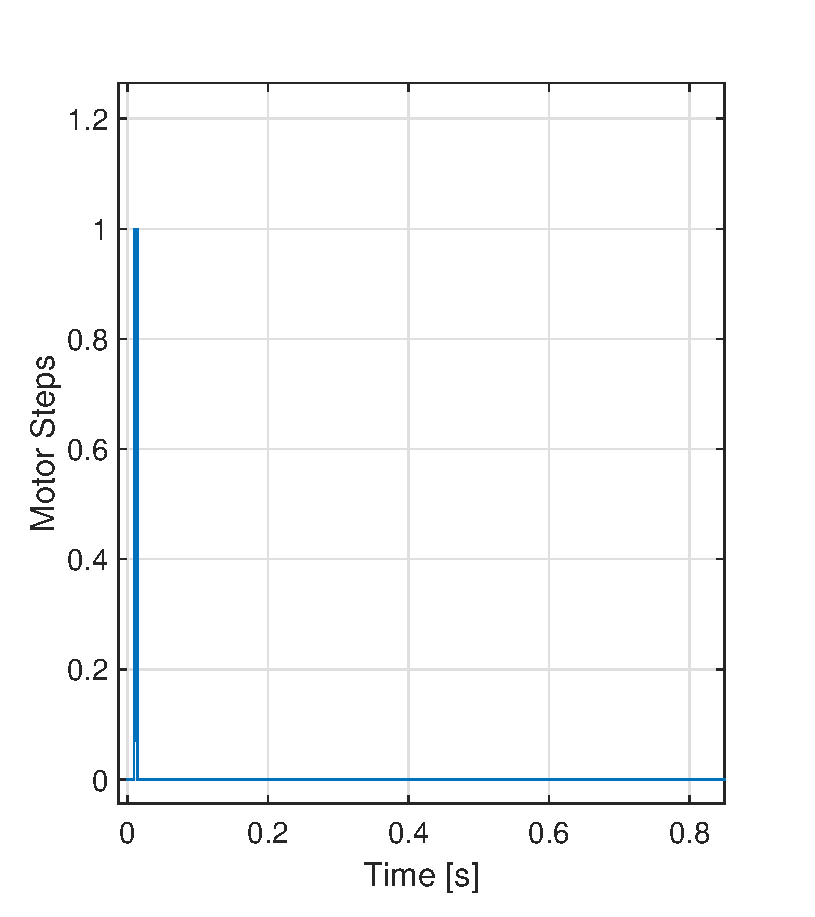
\includegraphics[width=0.46\textwidth, trim=0cm 0cm 1cm 0cm, clip=true]{fig/matlab/ff_impulse.eps}}
  \qquad
  \subfloat[][\label{fig:model_97} Impulse response from one step]{
  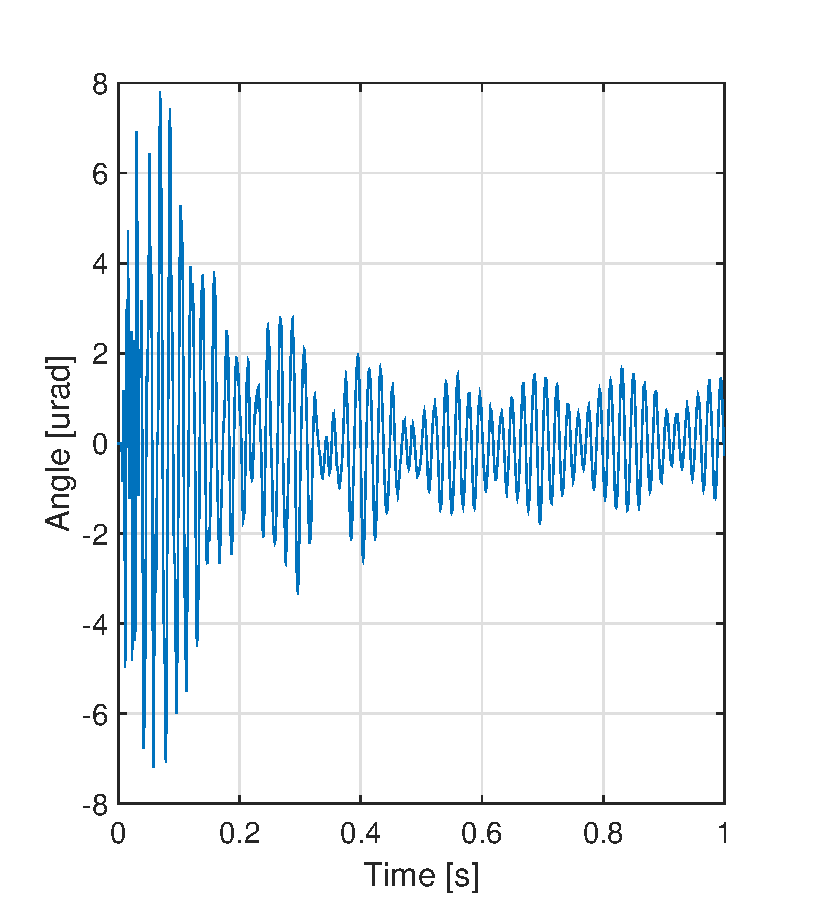
\includegraphics[width=0.46\textwidth, trim=0cm 0cm 1cm 0cm, clip=true]{fig/matlab/yaw_angle_mean_1_step_s.eps}}
  \caption{\label{fig:model_dist_high_order} Shows the input signal (a) and the mean of 50 acquired impulse responses (b) used in the identification.}
\end{figure}

\begin{figure}[h!]
  \centering %crop: left bottom right top
  \subfloat[][\label{fig:model_83} \abbrFFT at 0V ]{
  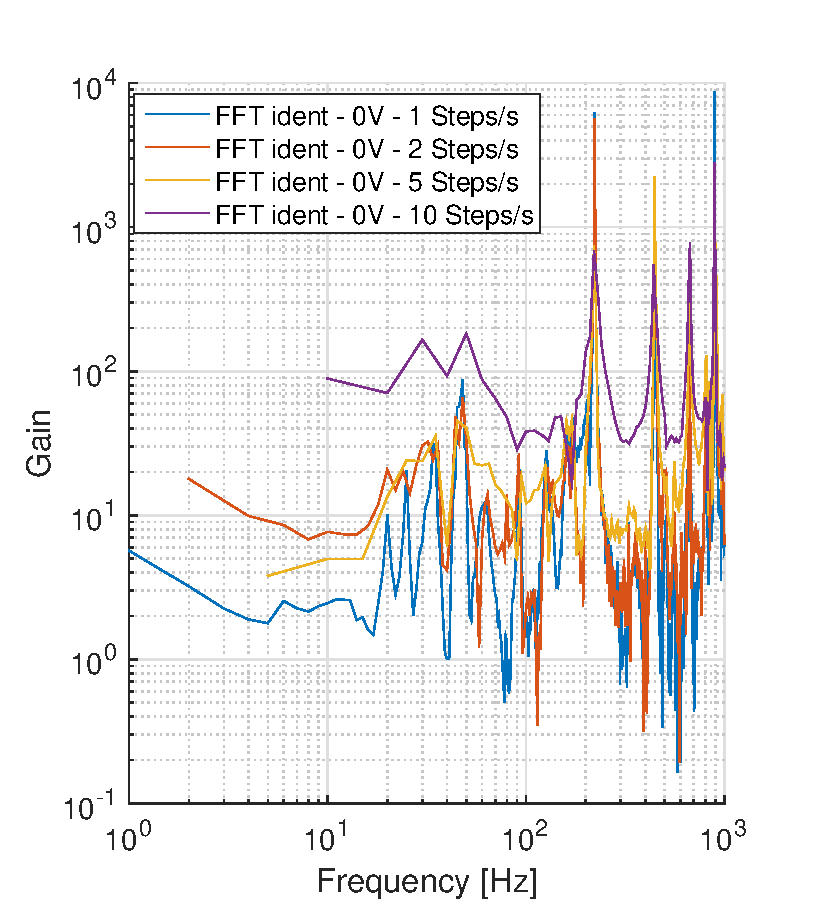
\includegraphics[width=0.46\textwidth, trim=0cm 0cm 0.9cm 0cm, clip=true]{fig/matlab/fft_mean_in_out_0V.eps}}
  \qquad
  \subfloat[][\label{fig:model_97} \abbrFFT at 3.25V]{
  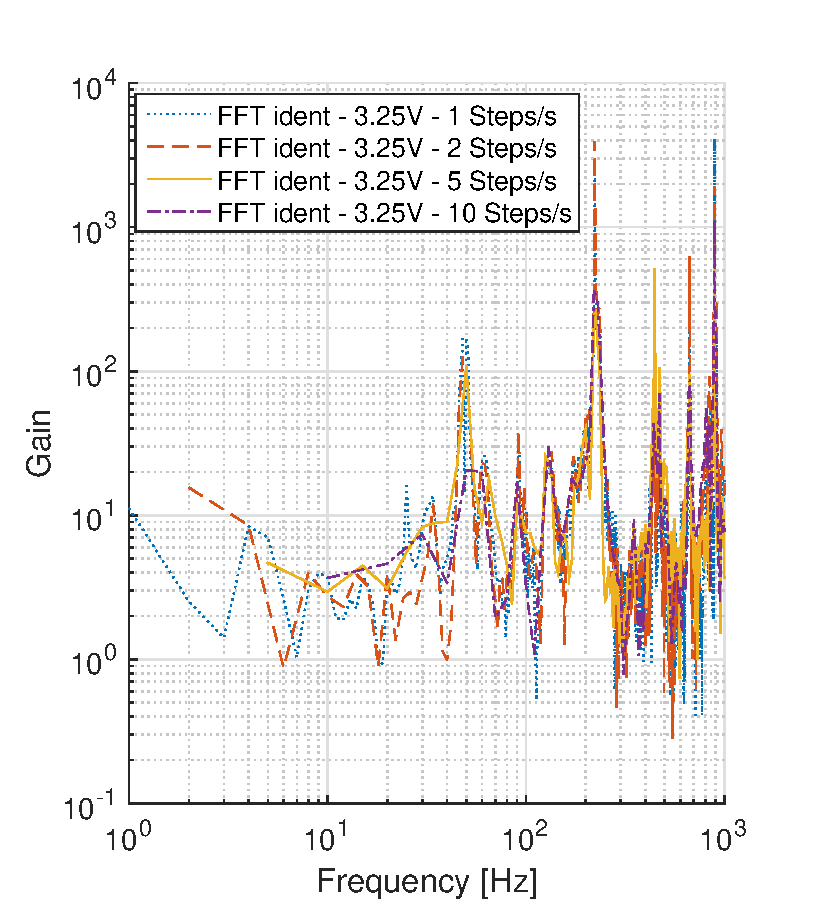
\includegraphics[width=0.46\textwidth, trim=0cm 0cm 0.9cm 0cm, clip=true]{fig/matlab/fft_mean_in_out_3V.eps}}
  \caption{\label{fig:model_dist_high_order} \abbrFFT of the response divided by the \abbrFFT of the impulse at two different voltages i.e. rotational positions, 0V - 0mrad (a) and 3.25 - 10mrad (b) with four different stepping speeds.}
\end{figure}

\begin{figure}[h!]
  \centering %crop: left bottom right top
  \subfloat[][\label{fig:model_83}\abbrFFT at 6.5V]{
  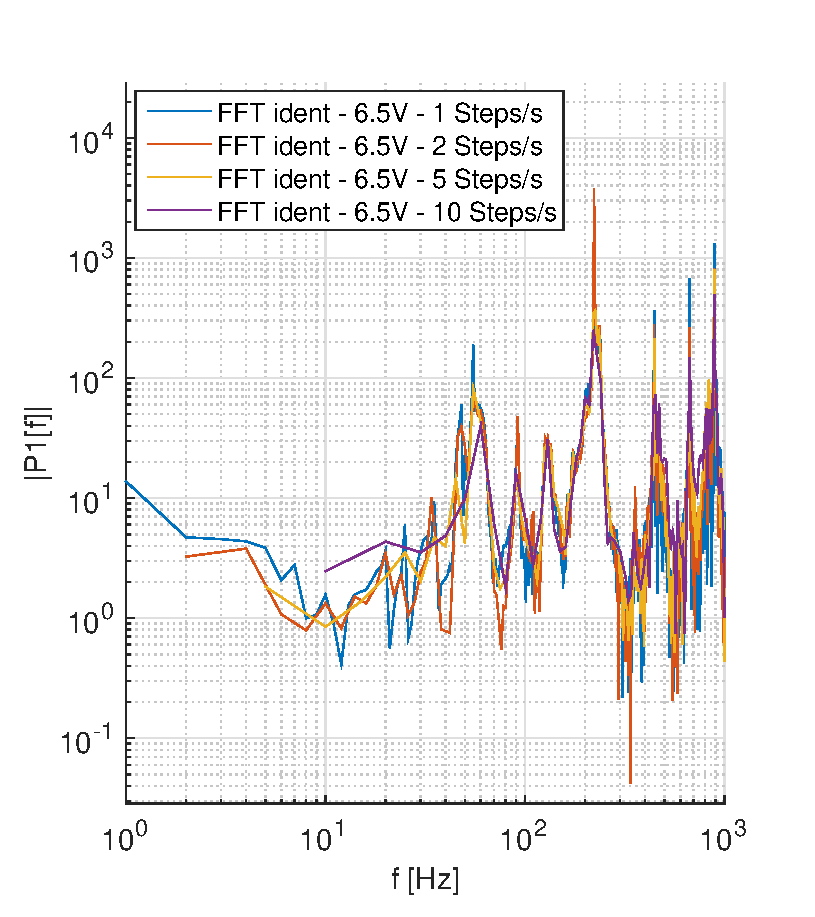
\includegraphics[width=0.46\textwidth, trim=0cm 0cm 1cm 0cm, clip=true]{fig/matlab/fft_mean_in_out_6_5V.eps}}
  \qquad
  \subfloat[][\label{fig:model_97}Identified model]{
  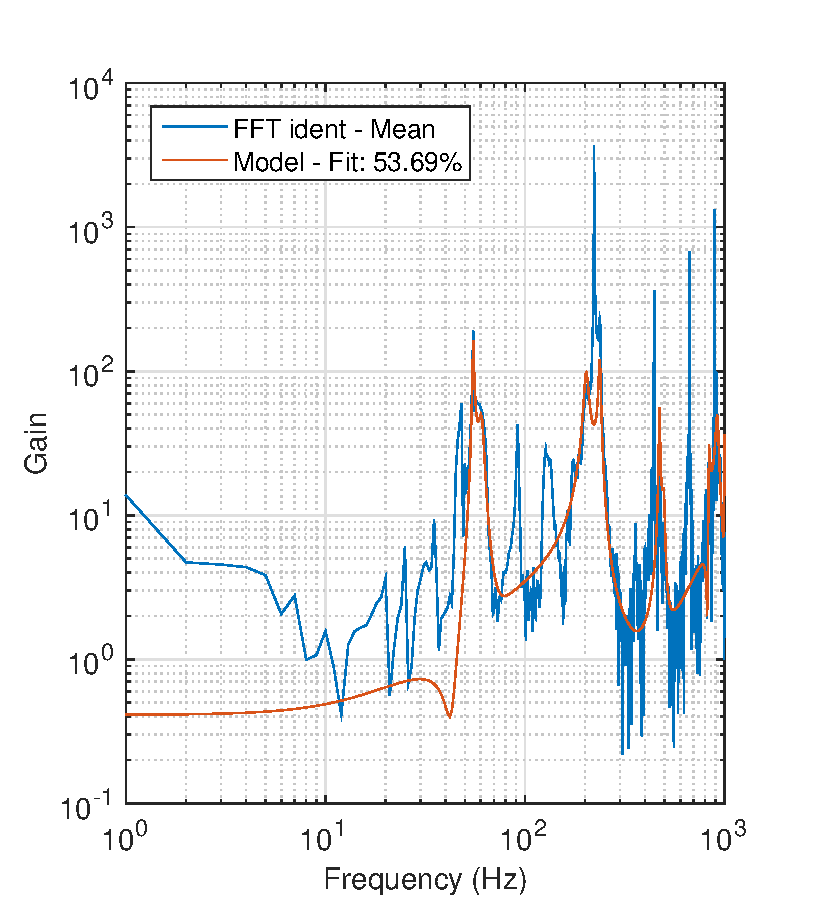
\includegraphics[width=0.46\textwidth, trim=0cm 0cm 1cm 0cm, clip=true]{fig/matlab/model_fit_1step_s.eps}}
  \caption{\label{fig:model_dist_high_order} Shows the \abbrFFT of the response divided by the \abbrFFT at 6.5V - 0mrad (a) at different speeds and the corresponding identified model (b).}
\end{figure}

\begin{figure}[h!]
  \centering %crop: left bottom right top
  \subfloat[][\label{fig:model_83} Mean as disturbance]{
  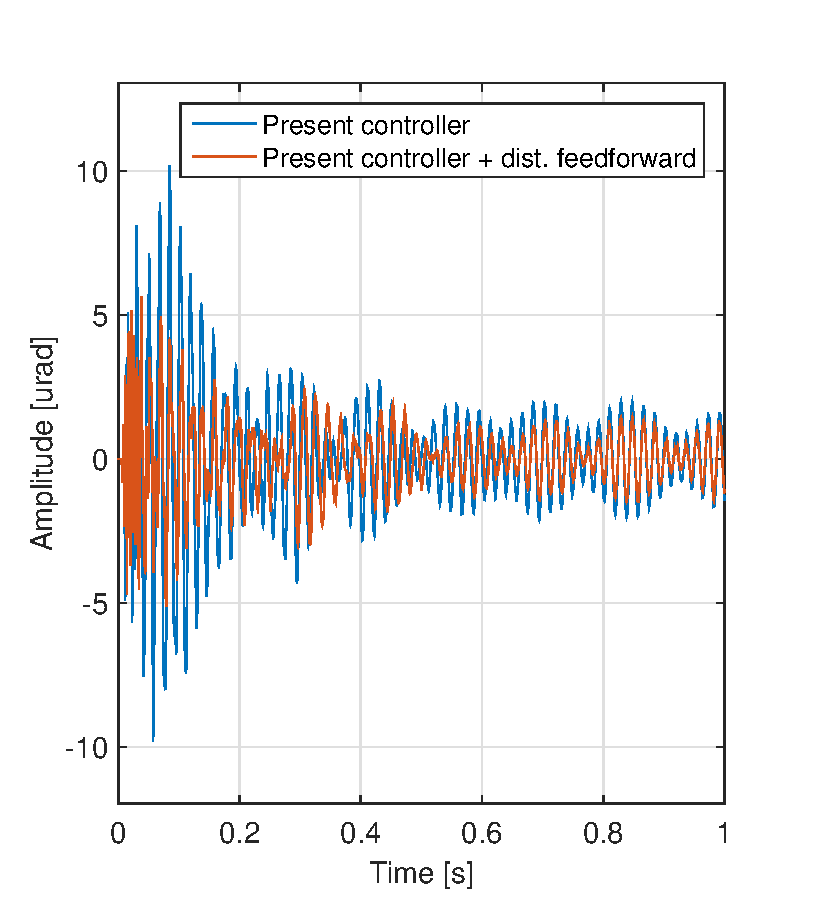
\includegraphics[width=0.46\textwidth, trim=0cm 0cm 1cm 0cm, clip=true]{fig/matlab/cancellation_1_step_s.eps}}
  \qquad
  \subfloat[][\label{fig:model_97} Acquired signal as disturbance ]{
  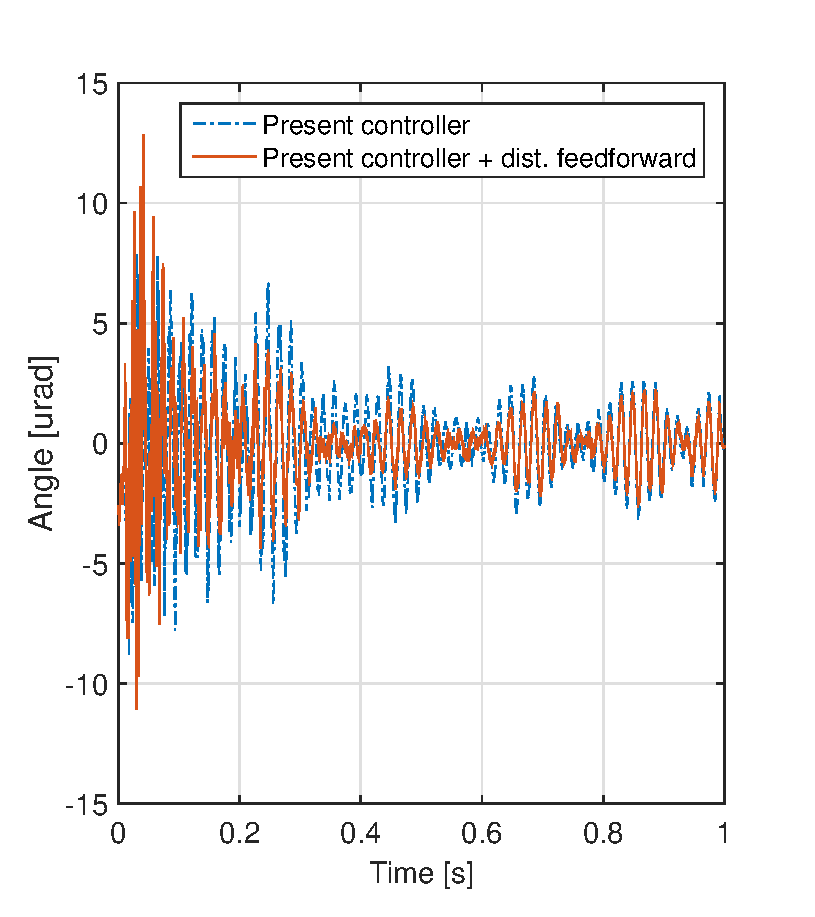
\includegraphics[width=0.46\textwidth, trim=0cm 0cm 1cm 0cm, clip=true]{fig/matlab/cancellation_1_step_s_real_dist.eps}}
  \caption{\label{fig:model_dist_high_order} Shows the effect of the feedforward disturbance cancellation with the mean of the acquired response added as disturbance (a) and one period of the acquired response added as disturbance (b).}
\end{figure}

\begin{table}[h!]
  \centering
  \begin{tabular}{| l | l | l | l | l |}
    \hline
      Speed & 1 step/s & 2 step/s & 5 step/s & 10 step/s\\ \hline
      $\sigma_{Present}$ & 2.15 & 2.23 & 3.90 & 3.76\\
      $\sigma_{Present + dist.FF.}$ & 1.19 & 2.04 & 2.06 & 2.59\\
    \hline
  \end{tabular}
  \caption{\label{tab:std} Standard deviations of the output with and without disturbance feedforward for the different speeds with the mean of the acquired response added as disturbance. The model used in the disturbance feedforward was identified from the 6.5V and 1step/s data.}
\end{table}




%
% \newpage
% \section{Experimental Results}
% \subsection{Setup}
% The experiments have been conducted on the considered rotational stage described in Section~\ref{sec:rotational_stage}. A National Instruments PXI communicates with the Collimator and the rotational stage, responsible for acquisition and control. To drive the rotational stage it outputs a voltage between [-1, 7.5] V, this is amplified by a linear amplifier with a gain of \unit{20}{\volt/\volt} resulting in a [-20, 150] V signal input on the rotational stage. The yaw angle, measured by the interferometric system is converted and sent to the PXI. The control loop is running at \unit{2}{\kilo\hertz}.
